%----------------------------------------------------------------------------------------------------------------
% Codificação: UTF-8
% LaTeX:  abnTeX2          
% ---------------------------------------------------------------------------------------------------------------


% CARREGA CLASSE PERSONALIZADA DA UTFPR--------------------------------------------------------------------------
\documentclass[%twoside,                   % Impressão em frente e verso
    	        oneside,                   % Impressão apenas frente
]{configuracoes/utfpr-abntex2}


% INCLUI ARQUIVOS DE CONFIGURAÇÕES-------------------------------------------------------------------------------
% REFERÊNCIAS------------------------------------------------------------------
\usepackage[%
    alf,
    abnt-emphasize=bf,
    bibjustif,
    recuo=0cm,
    abnt-url-package=url,       % Utiliza o pacote url
    abnt-refinfo=yes,           % Utiliza o estilo bibliográfico abnt-refinfo
    abnt-etal-cite=3,
    abnt-etal-list=3,
    abnt-thesis-year=final
]{abntex2cite}                  % Configura as citações bibliográficas conforme a norma ABNT

% PACOTES----------------------------------------------------------------------
\usepackage[utf8]{inputenc}                                 % Codificação do documento
\usepackage[T1]{fontenc}                                    % Seleção de código de fonte
\usepackage{booktabs}                                       % Réguas horizontais em tabelas
\usepackage{color, colortbl}                                % Controle das cores
\usepackage{float}                                          % Necessário para tabelas/figuras em ambiente multi-colunas
\usepackage{graphicx}                                       % Inclusão de gráficos e figuras
\usepackage{icomma}                                         % Uso de vírgulas em expressões matemáticas
\usepackage{indentfirst}                                    % Indenta o primeiro parágrafo de cada seção
\usepackage{microtype}                                      % Melhora a justificação do documento
\usepackage{multirow, array}                                % Permite tabelas com múltiplas linhas e colunas
\usepackage{subeqnarray}                                    % Permite subnumeração de equações
\usepackage{lastpage}                                       % Para encontrar última página do documento
\usepackage{verbatim}                                       % Permite apresentar texto tal como escrito no documento, ainda que sejam comandos Latex
\usepackage{amsfonts, amssymb, amsmath}                     % Fontes e símbolos matemáticos
\usepackage[algoruled, portuguese]{algorithm2e}             % Permite escrever algoritmos em português
%\usepackage[scaled]{helvet}                                % Usa a fonte Helvetica
\usepackage{times}                                          % Usa a fonte Times
%\usepackage{palatino}                                      % Usa a fonte Palatino
%\usepackage{lmodern}                                       % Usa a fonte Latin Modern
\usepackage[bottom]{footmisc}                               % Mantém as notas de rodapé sempre na mesma posição
\usepackage{ae, aecompl}                                    % Fontes de alta qualidade
\usepackage{latexsym}                                       % Símbolos matemáticos
\usepackage{lscape}                                         % Permite páginas em modo "paisagem"
%\usepackage{picinpar}                                      % Dispor imagens em parágrafos
%\usepackage{scalefnt}                                      % Permite redimensionar tamanho da fonte
%\usepackage{subfig}                                        % Posicionamento de figuras
%\usepackage{upgreek}                                       % Fonte letras gregas

% Redefine a fonte para uma fonte similar a Arial (fonte Helvetica)
\renewcommand*\familydefault{\sfdefault}

% CONFIGURAÇÕES DE APARÊNCIA DO PDF FINAL--------------------------------------
\makeatletter
\hypersetup{%
    portuguese,
    colorlinks=true,   % true: "links" coloridos; false: "links" em caixas de texto
    linkcolor=blue,    % Define cor dos "links" internos
    citecolor=blue,    % Define cor dos "links" para as referências bibliográficas
    filecolor=blue,    % Define cor dos "links" para arquivos
    urlcolor=blue,     % Define a cor dos "hiperlinks"
    breaklinks=true,
    pdftitle={\@title},
    pdfauthor={\@author},
    pdfkeywords={abnt, latex, abntex, abntex2}
}
\makeatother

% ALTERA O ASPECTO DA COR AZUL--------------------------------------------------
\definecolor{blue}{RGB}{41,5,195}

% REDEFINIÇÃO DE LABELS---------------------------------------------------------
\renewcommand{\algorithmautorefname}{Algoritmo}
\def\equationautorefname~#1\null{Equa\c c\~ao~(#1)\null}

% CRIA ÍNDICE REMISSIVO---------------------------------------------------------
\makeindex

% HIFENIZAÇÃO DE PALAVRAS QUE NÃO ESTÃO NO DICIONÁRIO---------------------------
\hyphenation{%
    qua-dros-cha-ve
    Kat-sa-gge-los
}



% INCLUI ARQUIVOS DO TRABALHO DE CONCLUSÃO DE CURSO (PRÉ-TEXTUAIS, TEXTUAIS, PÓS-TEXTUAIS)-----------------------

% INSERE CAPA E FOLHA DE ROSTO
% CAPA---------------------------------------------------------------------------------------------------

% ORIENTAÇÕES GERAIS-------------------------------------------------------------------------------------
% Caso algum dos campos não se aplique ao seu trabalho, como por exemplo,
% se não houve coorientador, apenas deixe vazio.
% Exemplos: 
% \coorientador{}
% \departamento{}

% DADOS DO TRABALHO--------------------------------------------------------------------------------------
\titulo{Desenvolvimento de Mesa de Luz Interativa para Experimento de Ciências para Crianças}
\titleabstract{Title in English}
\autor{Wendeurick Emerick Silverio}
\autorcitacao{SILVERIO, Wendeurick} % Sobrenome em maiúsculo
\local{Curitiba}
\data{2018}

% NATUREZA DO TRABALHO-----------------------------------------------------------------------------------
% Opções: 
% - Trabalho de Conclusão de Curso (se for Graduação)
% - Dissertação (se for Mestrado)
% - Tese (se for Doutorado)
% - Projeto de Qualificação (se for Mestrado ou Doutorado)
\projeto{Trabalho de Conclusão de Curso}

% TÍTULO ACADÊMICO---------------------------------------------------------------------------------------
% Opções:
% - Bacharel ou Tecnólogo (Se a natureza for Trabalho de Conclusão de Curso)
% - Mestre (Se a natureza for Dissertação)
% - Doutor (Se a natureza for Tese)
% - Mestre ou Doutor (Se a natureza for Projeto de Qualificação)
\tituloAcademico{Engenheiro Eletricista}

% ÁREA DE CONCENTRAÇÃO E LINHA DE PESQUISA---------------------------------------------------------------
% Se a natureza for Trabalho de Conclusão de Curso, deixe ambos os campos vazios
% Se for programa de Pós-graduação, indique a área de concentração e a linha de pesquisa
\areaconcentracao{}
\linhapesquisa{}

% DADOS DA INSTITUIÇÃO-----------------------------------------------------------------------------------
% Se a natureza for Trabalho de Conclusão de Curso, coloque o nome do curso de graduação em "programa"
% Formato para o logo da Instituição: \logoinstituicao{<escala>}{<caminho/nome do arquivo>}
\instituicao{Universidade Federal do Paraná}
\departamento{DELT - Departamento de Engenharia Elétrica}
\programa{Curso de Engenharia Elétrica}
\logoinstituicao{0.2}{dados/figuras/logo-instituicao.jpg} 

% DADOS DOS ORIENTADORES---------------------------------------------------------------------------------
\orientador{Dr. James Alexandre Baraniuk}
%\orientador[Orientadora:]{Nome da orientadora}
\instOrientador{DELT - Departamento de Engenharia Elétrica}

\coorientador{}
%\coorientador[Coorientadora:]{Nome da coorientadora}
\instCoorientador{}

% FOLHA DE ROSTO--------------------------------------------------------------------------------------------------------

% TRABALHO DE CONCLUSÃO DE CURSO
 \preambulo{{\imprimirprojeto} apresentado ao {\imprimirprograma} da {\imprimirinstituicao}, como requisito parcial para a obtenção do título de {\imprimirtituloAcademico}.}

% DISSERTAÇÃO DE MESTRADO
% \preambulo{{\imprimirprojeto} apresentada ao Programa de \mbox{Pós-graduação} da {\imprimirinstituicao}, como requisito parcial para obtenção do título de {\imprimirtituloAcademico}.}

% TESE DE DOUTORADO
% \preambulo{{\imprimirprojeto} apresentada ao Programa de \mbox{Pós-graduação} da {\imprimirinstituicao}, como requisito parcial para a obtenção do título de {\imprimirtituloAcademico}.}

% PROJETO DE QUALIFICAÇÃO DE MESTRADO OU DOUTORADO
%\preambulo{{\imprimirprojeto} apresentado ao Programa de \mbox{Pós-graduação} da {\imprimirinstituicao}, como requisito parcial para a obtenção do título de {\imprimirtituloAcademico}.}

% OBSERVAÇÕES-----------------------------------------------------------------------------------------------------------
% Altere este arquivo APENAS comentando as linhas que não se aplicam ao tipo de trabalho acadêmico desejado.



\begin{document}

\pretextual
\imprimircapa                                               	           % Comando para imprimir Capa
\imprimirfolhaderosto{}                                     		   % Comando para imprimir Folha de rosto
% INSERE ELEMENTOS PRÉ-TEXTUAIS
%% DEDICATÓRIA------------------------------------------------------------------

\renewcommand{\dedicatorianame}{DEDICATÓRIA}

\begin{dedicatoria}

À memória de Thiago Borges Fonseca. 

\end{dedicatoria}
          			   % Dedicatória
%% AGRADECIMENTOS---------------------------------------------------------------

\begin{agradecimentos}[AGRADECIMENTOS]

Edite e coloque aqui os agradecimentos às pessoas e/ou instituições que contribuíram para a realização do trabalho.

É obrigatório o agradecimento às instituições de fomento à pesquisa que financiaram total ou parcialmente o trabalho, inclusive no que diz respeito à concessão de bolsas.

\end{agradecimentos}
        			   % Agradecimentos
%% EPÍGRAFE---------------------------------------------------------------------

\renewcommand{\epigraphname}{EPÍGRAFE}

\begin{epigrafe}

\textit{Gosto que tudo seja real e que tudo esteja certo;\\
E gosto porque assim seria, mesmo que eu não gostasse.\\
Por isso, se morrer agora, morro contente,\\
Porque tudo é real e tudo está certo.\\\\
(CAEIRO, Alberto (Fernando Pessoa), 1915).}

\end{epigrafe}

% OBSERVAÇÕES------------------------------------------------------------------
% Altere o texto para inserir a epígrafe do seu trabalho

              			   % Epígrafe
% RESUMO--------------------------------------------------------------------------------

\begin{resumo}[RESUMO]
\begin{SingleSpacing}

% Não altere esta seção do texto--------------------------------------------------------
\imprimirautorcitacao. \imprimirtitulo. \imprimirdata. \pageref {LastPage} f. \imprimirprojeto\ – \imprimirprograma, \imprimirinstituicao. \imprimirlocal, \imprimirdata.\\
%---------------------------------------------------------------------------------------

O presente trabalho refere-se ao desenvolvimento do protótipo de uma matriz de LED que será parte da exposição interativa ``Luz, Ciência e Emoção'', idealizada pela arquiteta Dra. Maristela Mitsuko Ono e pelo engenheiro Dr. James Alexandre Baraniuk. A matriz, chamada de ``Mesa de Bolinhas'', se enquadra no setor artístico da exposição, que traz experimentos envolvendo os conceitos de luz trabalhados nos ensinos pré-escolar e fundamental, e proporcionará uma experiência tangível-visual impactante aos observadores, causando deslumbramento e entusiamos através da interação com arte e tecnologia.
Entre os desafios do projeto, \textcolor{red}{TODO: falar sobre técnicas de contorno (debounce), endereçamento dos quase 400 canais de PWM, FSM}\\

\textbf{Palavras-chave}: Matriz de LED. Matriz de sensores. Arte generativa.

\end{SingleSpacing}
\end{resumo}

% OBSERVAÇÕES---------------------------------------------------------------------------
% Altere o texto inserindo o Resumo do seu trabalho.
% Escolha de 3 a 5 palavras ou termos que descrevam bem o seu trabalho 

             			   % Resumo em Português
% ABSTRACT--------------------------------------------------------------------------------

\begin{resumo}[ABSTRACT]
\begin{SingleSpacing}

% Não altere esta seção do texto--------------------------------------------------------
\imprimirautorcitacao. \imprimirtitleabstract. \imprimirdata. \pageref {LastPage} f. \imprimirprojeto\ – \imprimirprograma, \imprimirinstituicao. \imprimirlocal, \imprimirdata.\\
%---------------------------------------------------------------------------------------

\textcolor{red}{TODO: resumo em língua extrangeira}.\\

\textbf{Keywords}: Word. Second Word. Another word.

\end{SingleSpacing}
\end{resumo}

% OBSERVAÇÕES---------------------------------------------------------------------------
% Altere o texto inserindo o Abstract do seu trabalho.
% Escolha de 3 a 5 palavras ou termos que descrevam bem o seu trabalho 
             		           % Resumo em Inglês
% Lista de Figuras----------------------------------------------------------------

\pdfbookmark[0]{\listfigurename}{lof}
\listoffigures*
\cleardoublepage

% OBSERVAÇÕES---------------------------------------------------------------------
% Este arquivo não precisa de ser alterado, pois a lista é gerada automaticamente.
   % Lista de Figuras
% LISTA DE QUADROS----------------------------------------------------------------

\renewcommand{\listofquadrosname}{LISTA DE QUADROS}

\pdfbookmark[0]{\listofquadrosname}{loq}
\listofquadros*
\cleardoublepage

% OBSERVAÇÕES---------------------------------------------------------------------
% Este arquivo não necessita de ser editado. A lista é gerada automaticamente.
   % Lista de Quadros
% LISTA DE TABELAS-------------------------------------------------------------

\pdfbookmark[0]{\listtablename}{lot}
\listoftables*
\cleardoublepage

% OBSERVAÇÕES-------------------------------------------------------------------
% Este arquivo não precisa ser alterado, pois a lista é gerada automaticamente.
         		   % Lista de Tabelas
% LISTA DE ABREVIATURAS E SIGLAS----------------------------------------------------------
\begin{siglas}
    \item[ADC] do inglês \emph{Analog to Digital Converter}
    \item[API] do inglês \emph{Application Programming Interface}
    \item[CPU] do inglês \emph{Central Processing Unit}
    \item[FIFO] do inglês \emph{First In, First Out}
    \item[FSM] do inglês \emph{Finite-state Machine}
    \item[GPIO] do inglês \emph{General Purpose Input/Output}
    %\item[IC] Iniciação Científica
    %\item[IV] Radiação Infravermelha
    \item[LDR] do inglês \emph{Light Dependent Resistor}
    \item[LED] do inglês \emph{Light Emitting Diode}
    \item[MISO] do inglês \emph{Master Input Slave Output, or Master In Slave Out}
    \item[MOSI] do inglês \emph{Master Output Slave Input, or Master Out Slave In}
    \item[MuMa] Museu de Arte Municipal
    \item[NRZ] do inglês \emph{Non-return-to-zero}
    \item[OTA] do inglês \emph{Over-the-air}
    \item[PCI] Placa de Circuito Impresso
    \item[PIBIC] Programa Institucional de Bolsas de Iniciação Científica
    \item[PWM] do inglês \emph{Pulse Width Modulation}
    \item[RAM] do inglês \emph{Random Access Memory}
    \item[RGB] Sistema de cores aditivas, do inglês \emph{Red}, \emph{Green} e \emph{Blue}
    \item[SCLK] do inglês \emph{Serial Clock}
    \item[SMD] do inglês \emph{Surface Mounting Device}
    \item[SPIFFS] do inglês \emph{SPI Flash File System}
    \item[SS] do inglês \emph{Slave Select}
    \item[TCP] do inglês \emph{Transmission Control Protocol}
    \item[TJB] Transistor de Junção Bipolar
    %\item[TTL] do inglês \emph{Transistor-Transistor Logic}
    \item[UART] do inglês \emph{Universal Asynchronous Receiver-Transmitter}
    \item[UDP] do inglês \emph{User Datagram Protocol}
    \item[UFPR] Universidade Federal do Paraná
    \item[UNESCO] Organização das Nações Unidas para a Educação, a Ciência e a Cultura
    \item[USB] do inglês \emph{Universal Serial Bus}
\end{siglas}

% OBSERVAÇÕES-----------------------------------------------------------------------------
% Altere a lista acima para definir os acrônimos e siglas utilizados neste trabalho
          		   % Lista de Abreviaturas e Siglas
% LISTA DE SÍMBOLOS------------------------------------------------------------

\begin{simbolos}
    \item[$ \Omega $] Unidade de medida da resistência elétrica
    \item[$ \lambda $] Comprimento de onda
\end{simbolos}

% OBSERVAÇÕES-------------------------------------------------------------------
% Altere a lista acima para definir os símbolos utilizados no trabalho
        		   % Lista de Símbolos
% LISTA DE ALGORITMOS----------------------------------------------------------

\newcommand{\algoritmoname}{Algoritmo}
\renewcommand{\listalgorithmcfname}{LISTA DE ALGORITMOS}

\floatname{algocf}{\algoritmoname}
\newlistof{listofalgoritmos}{loa}{\listalgoritmoname}
\newlistentry{algocf}{loa}{0}

\counterwithout{algocf}{chapter}
\renewcommand{\cftalgocfname}{\algoritmoname\space}
\renewcommand*{\cftalgocfaftersnum}{\hfill--\hfill}

\pdfbookmark[0]{\listalgorithmcfname}{loa}
\listofalgorithms
\cleardoublepage

% OBSERVAÇÕES------------------------------------------------------------------
% Este arquivo não precisa ser alterado, pois a lista é gerada automaticamente.
   % Lista de Algoritmos
% SUMÁRIO----------------------------------------------------------------------

\renewcommand{\contentsname}{SUMÁRIO}

\pdfbookmark[0]{\contentsname}{toc}
\tableofcontents*
\cleardoublepage

% OBSERVAÇÕES-------------------------------------------------------------------
% Este arquivo não precisa ser alterado, pois o sumário é gerado automaticamente.
               			   % Sumário

\textual
% INSERE ELEMENTOS TEXTUAIS
% INTRODUÇÃO-------------------------------------------------------------------

\chapter{INTRODUÇÃO}
\label{chap:introducao}

  A luz exerce um papel essencial no nosso cotidiano e está presente das mais diversas formas: iluminação, medicina, pesquisas científicas, geração de energia, telecomunicações, educação, arte, cultura, etc. A Assembleia Geral das Nações Unidas proclamou o ano de 2015 como o Ano Internacional da Luz e das Tecnologias Baseadas na Luz \cite{resolucao-onu}, a fim de reconhecer tal importância para a vida dos cidadãos e para o desenvolvimento futuro da sociedade mundial. No ano da celebração, a UNESCO promoveu uma série de eventos por vários países \citeonline{eventos-unesco}, com o intuito de destacar que o aumento da consciência mundial e o fortalecimento do ensino da ciência e das tecnologias da luz são essenciais para abordar os desafios futuros e atuais, tais como o desenvolvimento sustentável, a energia e as comunicações, assim como para melhorar a qualidade de vida dos países menos desenvolvidos e dos em desenvolvimento.
  
  Baseada em tal iniciativa, a exposição Luz, Ciência e Emoção, idealizada pela arquiteta Dra. Maristela Mitsuko Ono e pelo engenheiro Dr. James Alexandre Baraniuk, traz experimentos envolvendo os conceitos de luz trabalhados nos ensinos pré-escolar e fundamental, cada um com seu grau de impressão aos sentidos. A (\autoref{fig:expo}) apresenta uma parte da mostra que ocorreu entre março e junho de 2017, no Museu de Arte Municipal, em Curitiba.
  
  \begin{figure}[H]%[!htb]
    \centering
    \caption{Parte da exposição ``Luz, Ciência e Emoção'', no MuMa}
    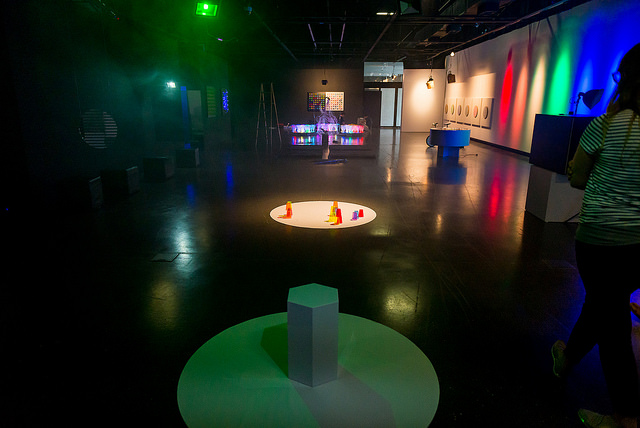
\includegraphics[width=0.95\textwidth]{./dados/figuras/expo}
    \fonte{(UFPR, 2017)}
    \label{fig:expo}
\end{figure}
  
  Dentre outros projetos que participou durante o Programa de Iniciação Científica \footnote{Projeto de Pesquisa: Luz, Ciência e Emoção: Exposição Interativa para Crianças (PIBIC Voluntária: 2016019080)}, o autor trabalhou na seção Matriz da Mesa de Bolinhas (\autoref{fig:mesa-sup}), projeto este que ocupará uma posição de destaque dentro da área artística da mostra. Trata-se de uma matriz de \emph{LEDs} interativa, composta por mais de 100 bolinhas de \emph{ping-pong}, cada uma sobre um correspondente par \emph{LED}-sensor reflexivo. Ela permite que o espectador ``pinte com luz'' ao passar a mão sobre a mesa, proporcionando uma experiência tangível-visual impactante, causando deslumbramento e entusiasmo através da arte e interação.
  
  O trabalho aqui proposto trata do desenvolvimento do \emph{hardware} e \emph{firmware} embarcado da seção Controle da mesa. Tal setor é responsável pela identificação e tratamento dos sinais de entrada e pelo acionamento da matriz de saída.

\begin{figure}[H]%[!htb]
    \centering
    \caption{Vista superior da mesa de Bolinhas}
    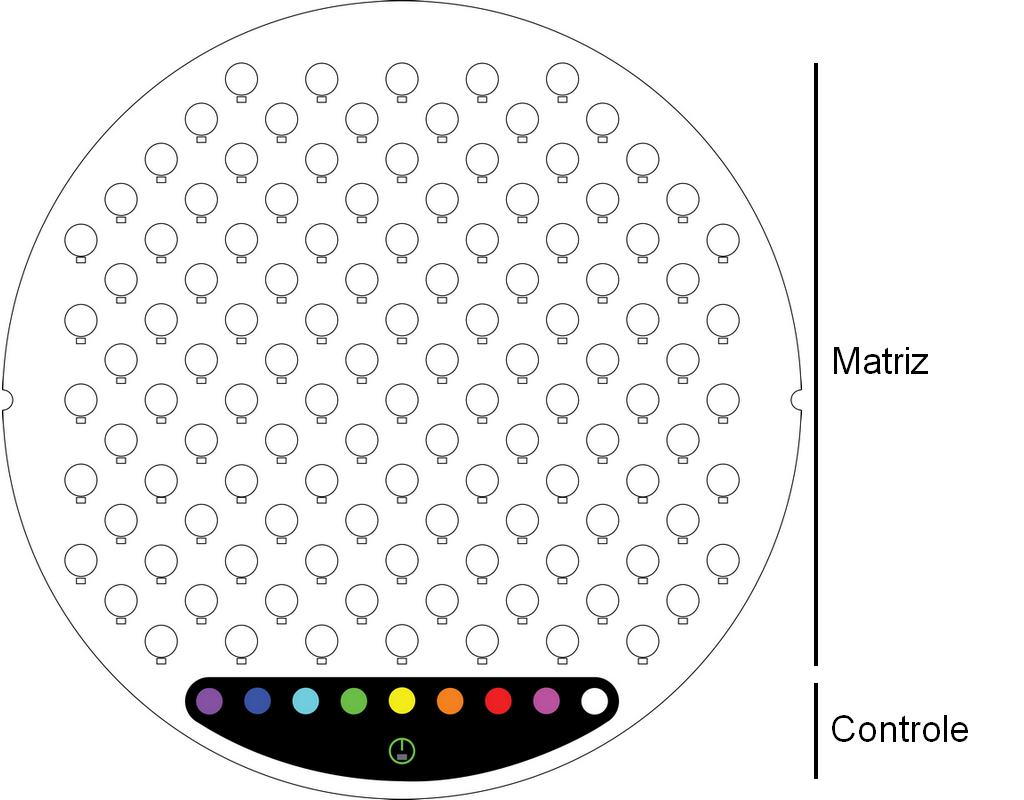
\includegraphics[width=0.7\textwidth]{./dados/figuras/mesa-cad}
    \fonte{(MITSUKO, 2016)}
    \label{fig:mesa-sup}
\end{figure}

\section{JUSTIFICATIVA}
\label{sec:justificativa}

  Sendo parte da exposição Luz, Ciência e Emoção, espera-se que o projeto fomente o envolvimento com a arte generativa e com as tecnologias envolvendo luz. Além de poder ser prestigiado durante a mostra, trata-se também de um projeto de código e \emph{hardware} abertos, que serão disponibilizados à comunidade para que possam ser estudados e adaptados às suas necessidades.

  Ademais, temas pouco explorados durante a graduação serão implementados, tais como técnica de contorno (\emph{debounce}, identificação de comandos reais sob contextos com ruído), padrão de \emph{design} em \emph{software} (FSM, máquina de estados finita) e geração de múltiplos canais de PWM.

\section{OBJETIVOS}
\label{sec:objetivos}

\subsection{OBJETIVO GERAL}
Finalizar o \emph{hardware} (seção Controle) e desenvolver o \emph{firmware} embarcado da Mesa de Bolinhas, apresentando um protótipo funcional do projeto.

\subsubsection{OBJETIVOS ESPECÍFICOS}
  \begin{itemize}
      \item Mapeamento da matriz de saída, onde cada \emph{LED} possa ser controlado individualmente;
      \item Mapeamento da matriz de entrada, onde cada sensor possa ser lido individualmente;
      \item \emph{Software} microcontrolado que gerencie a interface humano-máquina;
      \item Leiaute e montagem das Placas de Circuito Impresso;
      \item Integração da eletrônica com a mecânica do projeto.
  \end{itemize}
                		           % Introdução
% REVISÃO DE LITERATURA--------------------------------------------------------

\chapter{REVISÃO TEÓRICA}
\label{chap:fundamentacaoTeorica}

Este capítulo aborda alguns conceitos dos principais componentes e ferramentas utilizadas, bem como a especificação do projeto.

\section{PROJETO ARQUITETÔNICO}
\label{sec:matrizLed}

O projeto arquitetônico definiu a quantidade e a disposição de cada objeto. Ao todo, são 128 sensores e 129 pontos de luz, dispostos sob um tampo acrílico de 1m de diâmetro, conforme apresentado na \autoref{fig:tampo}.

\begin{figure}[H]
    \centering
    \caption{Disposição dos objetos na Mesa de Bolinhas}
    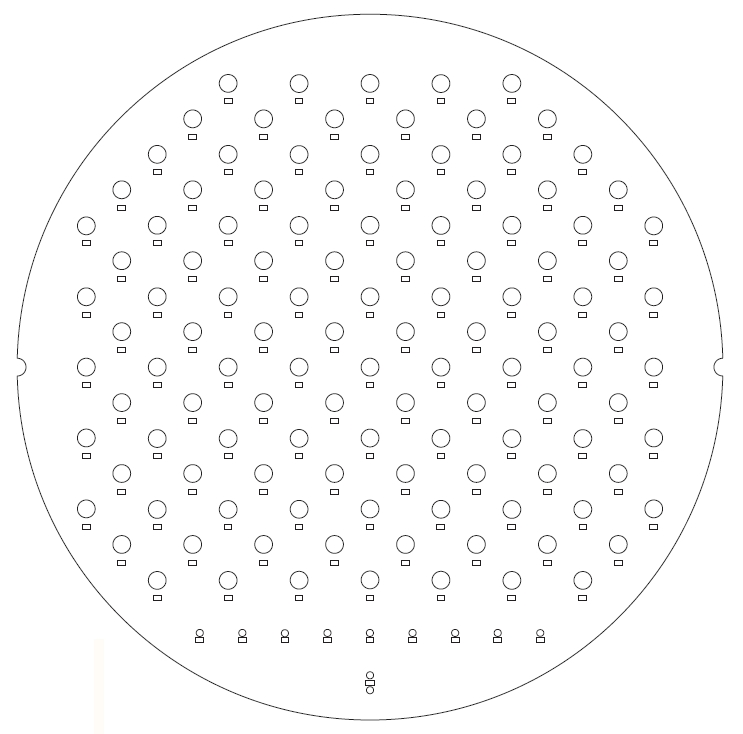
\includegraphics[width=0.8\textwidth]{./dados/figuras/tampo}
    \fonte{(MITSUKO, 2016)}
    \label{fig:tampo}
\end{figure}

A arquiteta também especifica que o funcionamento da mesa deve ser orientado a eventos, provenientes das seções Controle e Matriz (\autoref{fig:mesa-sup}):

\begin{itemize}[noitemsep]
    \item A mesa sai do modo ocioso ao manter-se a mão sobre a bolinha \emph{Power} por mais de 1s: acende-se o seletor de cores e a mesa passa a interpretar os demais comandos;
    \item Escolhe-se uma cor ao manter-se a mão sobre uma determinada bolinha do seletor de cores por mais de 1s;
    \item Ao passar a mão sobre uma determinada bolinha da seção Matriz, a mesma deve responder com a última cor escolhida;
    \item Uma bolinha da seção Matriz pode ser apagada se a ``cor'' escolhida tiver sido a da bolinha \emph{Power};
    \item Ao manter-se a mão por mais de 3s sobre a bolinha \emph{Power}, todas as bolinhas da seção Matriz devem ser apagadas; e
    \item Ao manter-se a mão por mais de 5s sobre a bolinha \emph{Power}, a mesa entra em modo ocioso: as bolinhas do seletor de cores são apagadas e a mesa passa a ignorar os comandos sobre a Matriz.
\end{itemize}

A partir da especificação acerca do funcionamento, notam-se alguns desafios do ponto de vista do eletrônico/lógico, tais como:

\begin{itemize}
    \item A disposição dos objetos e o tamanho da mesa;
    \item A capacidade de comandar individualmente 129 \emph{LEDs} coloridos (\emph{RGB}), ou seja $129 \times 3 = 387$ canais de cor;
    \item A capacidade de interpretar os níveis lógicos dos 128 sensores;
    \item A capacidade de responder, simultaneamente, aos comandos temporais provenientes de cada sensor.
\end{itemize}

A seleção dos componentes e das ferramentas foi baseada na especificação e nos desafios acima citados, e será discutida a seguir nas demais seções deste capítulo.

\section{SENSOR}
\label{sec:sensor}

A função do sensor é identificar a posição de um objeto, no caso, a mão do espectador, sobre o tampo acrílico, e para manter-se centrado nos objetivos do projeto arquitetônico, a definição do tipo de sensor foi baseada em dois pontos essenciais:

\begin{enumerate}[label=\Roman*.]
    \item O elemento principal do projeto é a luz que flui da bolinha de \emph{ping-pong};
    \item A exposição pode ser levada a diversos lugares e ser instalada nos mais variados ambientes, como museus, escolas, saguões e etc.
\end{enumerate}

A questão (I) implica que o sensor não deve irradiar ondas eletromagnéticas dentro do espectro visível, que vai de $400nm$ a $700nm$ \cite{fundafisica}. Já a questão (II) implica que a instalação será submetida a locais com diferentes graus de iluminação, portanto os sensores devem ser imunes à variação luminosa do ambiente.

Assim sendo, optou-se pelo sensor óptico reflexivo \emph{TCRT5000L}, apresentado na \autoref{fig:sensor}, cujas características relevantes para o projeto são apresentadas na \autoref{tab:sensor}.

\begin{figure}[H]
    \centering
    \caption{Sensor TCRT5000}
    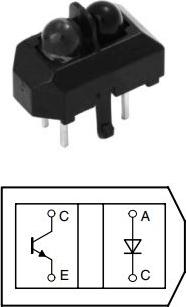
\includegraphics[width=0.24\textwidth]{./dados/figuras/sensor}
    \fonte{\citeonline{datasheet-sensor}}
    \label{fig:sensor}
\end{figure}

\begin{table}[H]
    \centering
    \caption[Principais características do sensor]{Principais características do sensor.
    \label{tab:sensor}}
    \begin{tabular}{|l|l|l|l|l|l|l|}
        \hline
        \textbf{Parâmetro} & \textbf{Condição} & \textbf{Símb.} & \textbf{Mín.} & \textbf{Típ.} & \textbf{Máx.} & \textbf{Unidade} \\     \hline
        \emph{LED} - Corrente direta &  & $I_{F}$ &  & 60 &  & mA \\ \hline
        \emph{LED} - Queda direta de tensão & $I_{F} = 60mA$ & $V_{F}$ &  & 1,25 & 1,5 & V \\ \hline
        \emph{LED} - Comprimento de onda & $I_{F} = 100mA$ & $\lambda_{P}$ & 940 &  &  & nm \\ \hline
        Sensor - Corrente de coletor & \begin{tabular}[c]{@{}l@{}}$@5V$,\\ $I_{F} = 10mA$,\\ $D=12mm$\end{tabular} & $I_{C}$ & 0,5 & 1 & 2,1 & mA \\ \hline
        \begin{tabular}[c]{@{}l@{}}Sensor - Queda de tensão entre\\ coletor-emissor na saturação\end{tabular} & \begin{tabular}[c]{@{}l@{}}$I_{F} = 10mA$, \\ $I_{C}=0,1mA$,\\ $D=12mm$\end{tabular} & $V_{CE_{sat}}$ &  &  & 0,4 & V \\ \hline
    \end{tabular}
    \fonte{\citeonline{datasheet-sensor}}
\end{table}


Trata-se de um sensor reflexivo infravermelho ($\lambda_{P}$), ou seja, opera fora do espectro visível, o que contorna a implicação da questão (I) apresentada anteriormente. Além disso, diferentemente de um sensor passivo, por exemplo um LDR, o TCRT5000 opera irradiando luz e, ademais, também contém filtro óptico embutido, absorvendo somente comprimentos de onda próximas a ($\lambda_{P}$). Essa duas características contornam a implicação da questão (II).

A saída transistorizada permite que o sensor seja interpretado de forma lógica. Sua aplicação (\autoref{fig:sensoraplicacao}) vai desde sensoriamento de \emph{encoders} e posições de ``fim de curso'' até detecção de papéis, cartões, fitas e etc. Foi escolhida a variante ``L'' (\emph{TCRT5000\textbf{L}}) por ser a versão com terminais estendidos.

\begin{figure}[H]
    \centering
    \caption{Aplicação do sensor TCRT5000}
    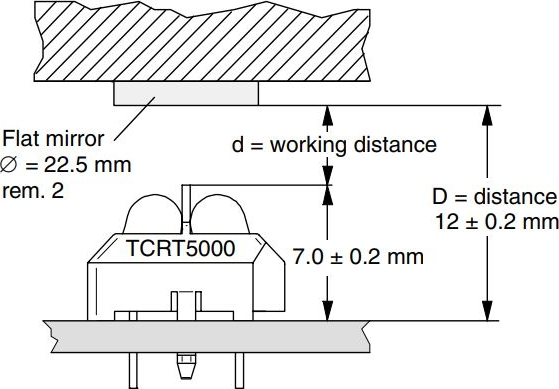
\includegraphics[width=0.5\textwidth]{./dados/figuras/sensor-op}
    \fonte{\citeonline{datasheet-sensor}}
    \label{fig:sensoraplicacao}
\end{figure}

\section{REGISTRADORES DE DESLOCAMENTO}
\label{sec:registradores}

A necessidade de interpretar individualmente os 128 sensores implica na mesma quantidade de entradas do circuito de processamento. Então, optou-se por lidar com entradas virtuais, através de um barramento serial, por meio de registradores de deslocamento. Dessa forma, com poucas GPIOs, o microcontrolador pode interpretar os níveis lógicos de todos os sensores conectados ao barramento.

Devido sua grande difusão no mercado, o registrador de deslocamento escolhido foi o 74HC165. A \autoref{fig:shift-register} apresenta o diagrama funcional do circuito integrado.

\begin{figure}[H]
    \centering
    \caption{Diagrama funcional do 74HC165}
    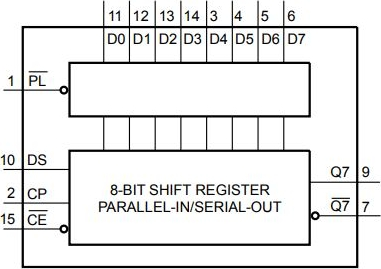
\includegraphics[width=0.5\textwidth]{./dados/figuras/shift-register}
    \fonte{\citeonline{datasheet-shift-register}}
    \label{fig:shift-register}
\end{figure}

Trata-se de um registrador de deslocamento com 8 entradas em paralelo ($D_{N}$) e saídas complementares ($Q_{7}$ e $\overline{Q_{7}}$) em serial. Basicamente, seu funcionamento (\autoref{fig:shift-temporal}) constitui-se na captura instantânea do nível lógico de suas entradas (borda de descida da Entrada Assíncrona de Carga Paralela, $\overline{P_{L}}$) e na transmissão desses valores através de deslocamento ordenado ($D_{7} \rightarrow D_{0}$) na saída serial ($Q_{7}$), nos eventos de borda de subida na entrada de \emph{clock} ($C_{P}$).

\begin{figure}[!htb]
    \centering
    \caption{Diagrama temporal do 74HC165}
    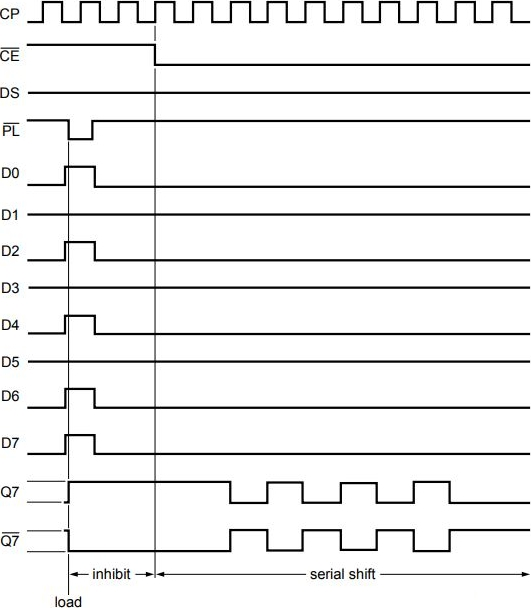
\includegraphics[width=0.6\textwidth]{./dados/figuras/shift-temporal}
    \fonte{\citeonline{datasheet-shift-register}}
    \label{fig:shift-temporal}
\end{figure}

%\section{TECLADO ADC}
%\label{sec:tecladoAD}

\section{LED}
\label{sec:led}

Para formar a matriz de saída, optou-se pelo LED WS2812S (\autoref{fig:ws2812}), um dispositivo em encapsulamento SMD5050 com controlador interno, o WS2811: um \emph{driver} especial para LEDs, com 3 saídas de 8 \emph{bits} de resolução, ou seja, pode-se gerar até 16777216 cores do padrão RGB. Esse controlador é muito utilizado em fitas de LEDs endereçáveis (\autoref{fig:strip}), pois permite a conexão de vários controladores em um mesmo barramento serial (protocolo NRZ), podendo-se controlar cada LED individualmente.

O fato de possuir um controlador embutido no próprio encapsulamento implica diretamente sobre o valor do LED, custando um pouco mais que o dobro do valor médio de outros LEDs RGBs mais simples. Apesar disso, o custo acaba sendo compensado pelos benefícios que o \emph{driver} proporciona.

\begin{figure}[!htb]
    \centering
    \caption{Vista aproximada do LED WS2812 e seu controlador interno}
    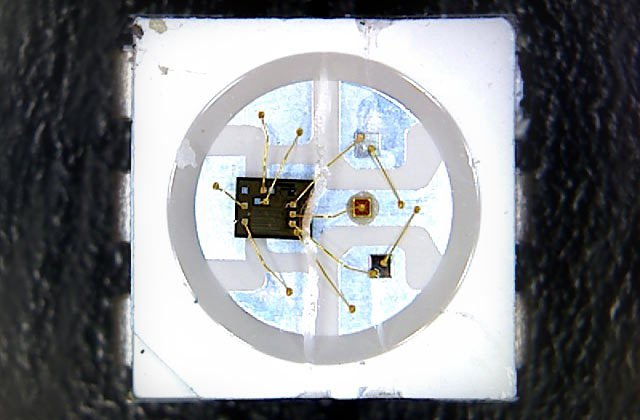
\includegraphics[width=0.65\textwidth]{./dados/figuras/ws2812}
    \fonte{\citeonline{adafruit}}
    \label{fig:ws2812}
\end{figure}

O modelo do LED já havia sido selecionada durante o Programa de Iniciação Científica que o autor participou, já sendo utilizado no circuito da matriz. No projeto aqui proposto, eles serão utilizados no seletor de cores, discutido no \autoref{chap:metodologia}.

\begin{figure}[H]
    \centering
    \caption{Fita de LED endereçável utilizando o WS2812}
    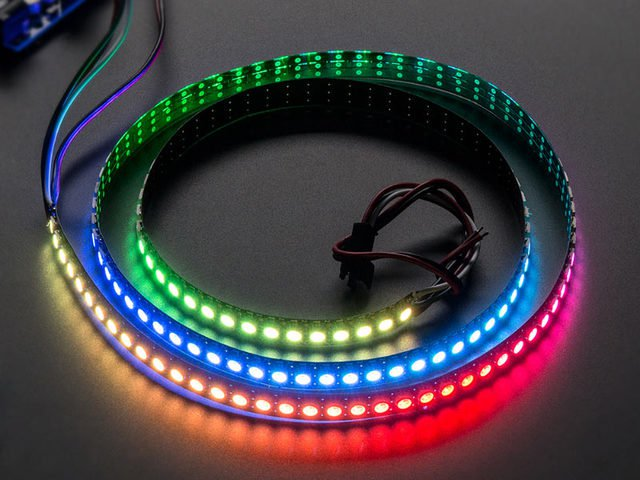
\includegraphics[width=0.5\textwidth]{./dados/figuras/strip}
    \fonte{\citeonline{adafruit}}
    \label{fig:strip}
\end{figure}

\textcolor{red}{TODO: consumo}

\section{BAKER CLAMP}
\label{sec:backerclamp}

Segundo \citeonline{theartofelectronics}, os mesmos efeitos que limitam o desempenho de amplificadores lineares em altas frequências (a combinação de capacitância de junção, capacitância de retorno e capacitância parasita) também impõem limitações de velocidade em circuitos digitais de alta frequência. A \autoref{fig:tjb} apresenta um amplificador ``emissor comum'', que pode atuar como uma chave inversora quando operado em corte e saturação, alimentado por uma fonte de pulsos com tempos de subida e descida extremamente curtos, e a \autoref{fig:curvatjb} apresenta uma curva típica sobre a carga ($R_{C}$) desse tipo de amplificador ao considerar as componentes parasitas. 

\begin{figure}[H]
    \centering
    \caption{Representação de uma chave inversora com TJB}
    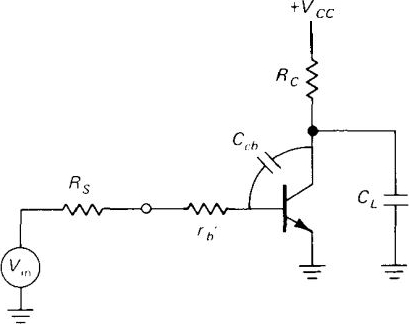
\includegraphics[width=0.45\textwidth]{./dados/figuras/tjb}
    \fonte{\cite{theartofelectronics}}
    \label{fig:tjb}
\end{figure}

\begin{figure}[H]
    \centering
    \caption{Forma de onda da chave inversora com TJB}
    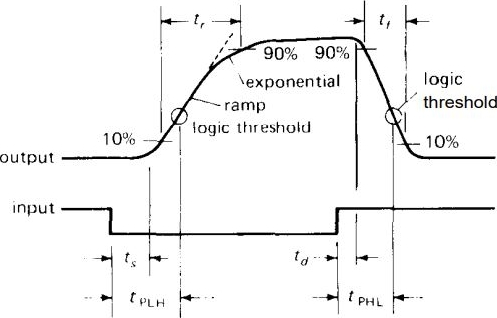
\includegraphics[width=0.6\textwidth]{./dados/figuras/curvatjb}
    \fonte{\cite{theartofelectronics}}
    \label{fig:curvatjb}
\end{figure}

Nota-se que, assim que a fonte estabelece o pulso em nível baixo, o transistor leva um certo tempo ($t_r$) para sair da saturação e alcançar o estado de corte. Esse comportamento deriva-se do acúmulo de carga ($C_{cb}$) entre o coletor e a base. Dependendo das características físicas do transistor e da aplicação, esse tempo de subida pode vir a prejudicar o desempenho da finalidade do circuito, como é o caso do conversor de nível lógico elaborado para a Mesa de Bolinhas (discutido no \autoref{chap:metodologia}).

Para mitigar tal efeito, \citeonline{theartofelectronics} propõem a inclusão de um diodo de \emph{clamping} (também conhecido por  ``Baker \emph{clamp}''), entre a base e o coletor do TJB (\autoref{fig:bakerclamp}). Esse diodo irá desviar a corrente de base quando o transistor estiver se aproximando da saturação e evitará sua saturação, uma vez que a queda direta de tensão do diodo, no caso um diodo Schottky, é menor que a da junção coletor-base. Dessa forma, o TJB pode entrar em corte mais rapidamente, pois o mesmo não chega a entrar no ponto de saturação profunda.

\begin{figure}[H]
    \centering
    \caption{Chave inversora com o diodo de ``Baker \emph{clamping}''}
    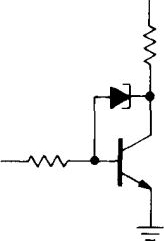
\includegraphics[width=0.25\textwidth]{./dados/figuras/bakerclamp}
    \fonte{\cite{theartofelectronics}}
    \label{fig:bakerclamp}
\end{figure}

\section{MICROCONTROLADOR}
\label{sec:microcontrolador}

O ESP8266 é o microcontrolador de entrada para a família de 32 bits da fabricante chinesa Espressif Systems. Produzido em escala a partir de 2014, essa família ganhou espaço na área de Internet das Coisas por ser um microcontrolador de baixo custo, de baixo consumo e com suporte à rede 802.11 (\emph{Wi-Fi}). A \autoref{tab:espec-microcontrolador} apresenta as principais especificações do microcontrolador e a \autoref{fig:esp-funcional} apresenta seu diagrama funcional. Cabe aqui ressaltar que toda a parte de radio-frequência é implementada por \emph{hardware}, simplificando o desenvolvimento de aplicações com comunicação sem fio.

\begin{table}[H]
    \centering
    \caption[Especificação do ESP8266]{Especificação do ESP8266.
    \label{tab:espec-microcontrolador}}
    \begin{tabular}{|l|l|}
    \hline
    Alimentação & 3,3\ V \\ \hline
    Consumo & $10\ \mu A - 170\ mA$ \\ \hline
    Memória Flash (externa) & 16\ MB máx. (512\ kB normal) \\ \hline
    CPU & Tensilica L106 32 bits \\ \hline
    \emph{Clock} & $80 - 160\ MHz$ \\ \hline
    RAM & $32\ kB - 80\ kB$ \\ \hline
    GPIOs & 17 (compartilhadas com outras funções) \\ \hline
    ADC & 1 canal (10 \emph{bits} de resolução) \\ \hline
    \emph{Wireless} & Estação, ponto de acesso ou ambos \\ \hline
    \end{tabular}
    \fonte{\cite{book-esp}}
\end{table}


\begin{figure}[!htb]
    \centering
    \caption{Diagrama funcional do ESP8266}
    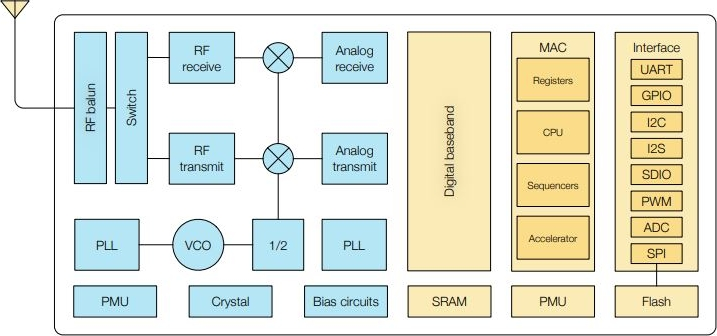
\includegraphics[width=0.9\textwidth]{./dados/figuras/esp-funcional}
    \fonte{\citeonline{datasheet-esp}}
    \label{fig:esp-funcional}
\end{figure}

Embora a comunicação sem fio não fizesse parte das especificações do projeto arquitetônico original, a equipe concordou com a possibilidade de implementá-la em uma aplicação futura. Esse foi o ponto decisivo para a escolha do ESP8266. Assim, a Mesa de Bolinhas poderá ganhar novas funcionalidades sem haver a necessidade de alteração no \emph{hardware}. Isso será discutido na \autoref{sec:trabalhosFuturos}.

Entre os diversos módulos que incluem o ESP8266, optou-se pelo ESP-12, por ser o que dispõe a maior quantidade de GPIOs (9 ao todo). A \autoref{fig:esp-12} apresenta sua placa. Convém salientar que este módulo já conta com memória \emph{Flash} (4MB) e antena \emph{microstrip}.

\begin{figure}[H]
    \centering
    \caption{Módulo ESP-12}
    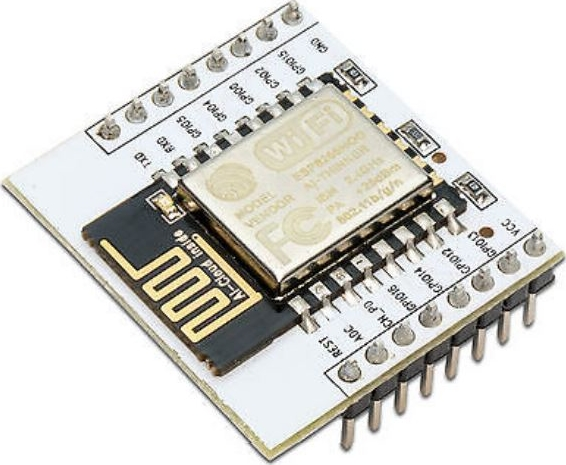
\includegraphics[width=0.4\textwidth]{./dados/figuras/esp-12}
    \fonte{\cite{book-esp}}
    \label{fig:esp-12}
\end{figure}

Por serem compartilhados entre aplicações do usuário e funcionalidades internas, alguns pinos possuem certas particularidades. Os resistores  \emph{pull-up/pull-down} (\autoref{fig:esp-12}) garantem o nível lógico de alguns pinos, porém outros necessitam de uma atenção especial, sobretudo os que definem o modo de funcionamento: operação normal ou modo de gravação, que será discutido no \autoref{chap:metodologia}. A \autoref{tab:pinoutesp} apresenta a pinagem do módulo ESP-12 e também a função interna cada pino.

\begin{table}[H]
    \centering
    \caption[Pinagem do módulo ESP-12]{Pinagem do módulo ESP-12.
    \label{tab:pinoutesp}}
\begin{tabular}{|l|l|}
\hline
\textbf{Pino} & \textbf{Descrição} \\ \hline
$V_{CC}$ & Alimentação 3,3\ V \\ \hline
GPIO 13 & Também usada pela SPI \\ \hline
GPIO 12 & Também usada pela SPI \\ \hline
GPIO 14 & Também usada pela SPI \\ \hline
GPIO 16 & Deve ser conectada ao RESET no modo \emph{Deep Sleep} \\ \hline
$CH_{PD}$ & \emph{Chip enable}: (0) desabilitado; (1) habilitado \\ \hline
ADC & Entrada do ADC \\ \hline
RESET & \emph{Reset} externo: (0) - \emph{reset}; (1) - normal \\ \hline
TXD & Transmissão da UART \\ \hline
RXD & Recepção da UART \\ \hline
GPIO 4 & GPIO regular \\ \hline
GPIO 5 & GPIO regular \\ \hline
GPIO 0 & Modo \emph{flah} se em nível baixo durante a inicialização \\ \hline
GPIO 2 & Deve estar em nível alto durante a inicialização \\ \hline
GPIO 15 & Deve estar em nível baixo durante a inicialização e gravação \\ \hline
GND & Terra \\ \hline
\end{tabular}
    \fonte{\cite{book-esp}}
\end{table}


\section{\emph{FRAMEWORK}}
\label{sec:framework}

Sming é um \emph{framework} de código aberto, nativo para a família de microcontroladores ESP8266, desenvolvido na linguagem {C++} e com foco em alta eficiência em desempenho e em uso de memória.

Diferente de outros \emph{frameworks} baseados em laço-infinito, a estrutura do Sming é baseada em eventos temporais: as tarefas do usuário são escaladas em uma tabela de tempo. Isso o aproxima de uma das funcionalidades de um Sitema Operacional de Tempo Real, embora não haja, obviamente, um gerenciamento de recursos. Porém, o fato de poder-se escalar as tarefas em uma janela de tempo simplifica a implementação da especificação deste projeto, uma vez que, basicamente, sua funcionalidade também é baseada em eventos temporais, como apresentado no começo do capítulo (\autoref{sec:matrizLed}).

Por tratar-se de uma plataforma de código aberto, este \emph{framework} conta com uma vasta contribuição da comunidade, com uma API de \emph{hardware} robusta e diversas bibliotecas nativas, tais como \emph{bootloader}, sistema de arquivos (SPIFFS), atualização sem fio de \emph{firmware} (OTA) e uma extensa pilha assíncrona de rede (TCP, UDP, \emph{WebSockets} e etc). Esses recursos são úteis para a continuidade do projeto, discutida na \autoref{sec:trabalhosFuturos}.

\section{FIFO}
\label{sec:fifo}

\textcolor{red}{TODO: revisão teórica FIFO}

\section{DEBOUNCE}
\label{sec:debounce}

Embora o funcionamento do sensor (\autoref{sec:sensor}) seja aparentemente simples - isto é, o transistor vai à saturação ao detectar um objeto; ou o transistor permanece em corte se não houver detecção - podem haver disparos falsos devido à oscilação do sinal durante a interação com a mesa. Essa oscilação é conhecida como \emph{bouncing}: trepidação do nível lógico durante a mudança de estado. A \autoref{fig:switch-bounce} apresenta um exemplo dessa oscilação, quando uma chave física passou do nível lógico alto para o baixo, ao ser pressionada.

\begin{figure}[H]
    \centering
    \caption{Oscilação do sinal de uma chave ao ser pressionada}
    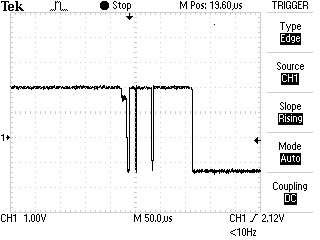
\includegraphics[width=0.6\textwidth]{./dados/figuras/bounce}
    \fonte{\citeonline{switch-debounce}}
    \label{fig:switch-bounce}
\end{figure}

Ainda que a Mesa de Bolinhas não conte com botões físicos, o efeito \emph{bouncing} pode vir a ocorrer em razão do limiar de detecção do sensor: o transistor de saída pode ficar operando, ainda que brevemente, no limite da interpretação do seu nível lógico. Para contornar tal situação, assim como nos casos de chaves físicas, será implementado um procedimento de \emph{debouncing}. \citeonline{debounceguide} cita diversas técnicas, desde descarte de tempo, filtros RC (resistor e capacitor), técnicas com \emph{latches} (\autoref{fig:srdebouncer}), entre outros, inclusive táticas via \emph{software}.

\begin{figure}[H]
    \centering
    \caption{Exemplo de circuito de \emph{debounce} com \emph{latches}}
    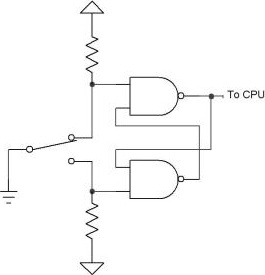
\includegraphics[width=0.4\textwidth]{./dados/figuras/srdebouncer}
    \fonte{\citeonline{debounceguide}}
    \label{fig:srdebouncer}
\end{figure}

No caso da Mesa de Bolinhas, não conviria implementar os modelos de  \emph{debouncing} por \emph{hardware}, pois implicaria diretamente no custo do projeto, não só pelo custo dos componentes, mas também pela área de placa ocupada, e também na complexidade do leiaute da PCI. Então, optou-se por implementar uma técnica de contorno via \emph{firmware}. Com isso, não há necessidade de adicionar componentes auxiliares ao circuito dos sensores e registradores de deslocamento. Trata-se de uma técnica baseada em ``histerese temporal'', onde a referência virtual altera-se de estado somente quando o nível de seu respectivo sensor já estiver estabilizado durante N milissegundos. A implementação dessa técnica será desenvolvida no \autoref{chap:metodologia}.
         % Revisão de Literatura
% METODOLOGIA------------------------------------------------------------------

\chapter{DESENVOLVIMENTO}
\label{chap:metodologia}

\textcolor{red}{TODO: intro}

Este capítulo aborda o desenvolvimento do \emph{hardware} do projeto, 

\section{CONCEPÇÃO DO PROJETO}
\label{sec:concepcao}

Com base no projeto arquitetônico e a partir do levantamento das tecnologias disponíveis e viáveis (sobretudo pelo custo e pela difusão no mercado), foram definidos os componentes e técnicas a serem utilizadas no projeto eletrônico, cujo diagrama geral é apresentado na \autoref{fig:diagramageral}.

\begin{figure}[H]
    \centering
    \caption{Diagrama geral do projeto eletrônico}
    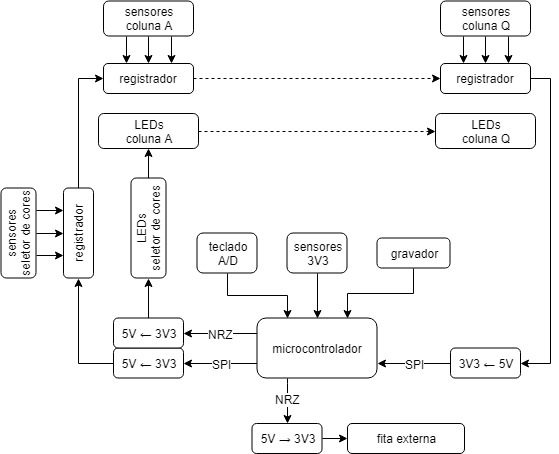
\includegraphics[width=0.8\textwidth]{./dados/figuras/diagrama}
    \fonte{(O AUTOR, 2018)}
    \label{fig:diagramageral}
\end{figure}

A partir do projeto arquitetônico (\autoref{fig:mesa-sup}), que é segmentado em duas partes: Matriz (interação) e Controle (seletor de cores), o projeto eletrônico também foi organizado em 3 subdivisões: Matriz, Interface e Controlador, apresentadas na \autoref{fig:subsecoes}. Dessa forma, pôde-se dar andamento ao projeto por meio de etapas, onde cada fase pode ser considerada um projeto íntegro por si só.

\begin{figure}[H]
    \centering
    \caption{As 3 subseções principais do projeto eletrônico}
    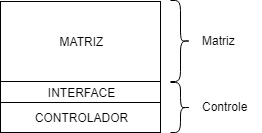
\includegraphics[width=0.40\textwidth]{./dados/figuras/secoes}
    \fonte{(O AUTOR, 2018)}
    \label{fig:subsecoes}
\end{figure}

As subdivisões têm funções bem definidas, apresentadas logo abaixo, e serão discutidas neste mesmo capítulo nos tópicos a seguir.

\begin{itemize}
    \item \textbf{Matriz:} é o setor que pode ser ``pintado com luz'', que contém os LEDs e os sensores de interação. É inteiramente comandada pelo Controlador, através da Interface;
    \item \textbf{Interface:} interliga as subseções Matriz e Controlador: captura e propaga o sinal dos sensores, através dos registradores de deslocamento, e forma a ligação sequencial do barramento dos LEDs;
    \item \textbf{Controlador:} processa todos os LEDs e sensores da mesa. Contém também os LEDs e os sensores do seletor de cores, a parte de processamento, os conversores de nível lógico e os periféricos de gravação e depuração.
\end{itemize}

%\textcolor{red}{TODO: especificações, tensão}

%\textcolor{red}{TODO: software}

\section{PROJETO DA MATRIZ}
\label{sec:matriz}

O projeto da Matriz foi concebido durante o Programa de Iniciação Científica do qual o autor participou. Nele, o desafio foi o de contemplar todas as 118 bolinhas de \emph{ping-pong} desta seção (e seus respectivos pares sensor-LED), visando robustez e o menor custo.

Para tal, foi definido que a matriz seria arranjada em 17 colunas verticais, conforme apresentado na \autoref{fig:placas-matriz-colunas}. Consequentemente, devido à disposição dos objetos (determinada pelo projeto arquitetônico), essas colunas poderiam conter 5, 6, 7 ou 8 bolinhas e, para abrangê-las da maneira mais proveitosa, as colunas foram combinadas por módulos (placas) de 2 ou 3 bolinhas.

Em geral, as empresas fabricantes de placas de circuito impresso consideram cada modelo de placa como um projeto, devido ao corte do painel, procedimento para os testes elétricos e etc. Assim, se utilizando de apenas 2 modelos de placa, foi possível reduzir o custo do projeto sem dispensar a robustez que as PCIs proporcionam.

\begin{figure}[H]
    \centering
    \caption{Disposição das placas da Matriz}
    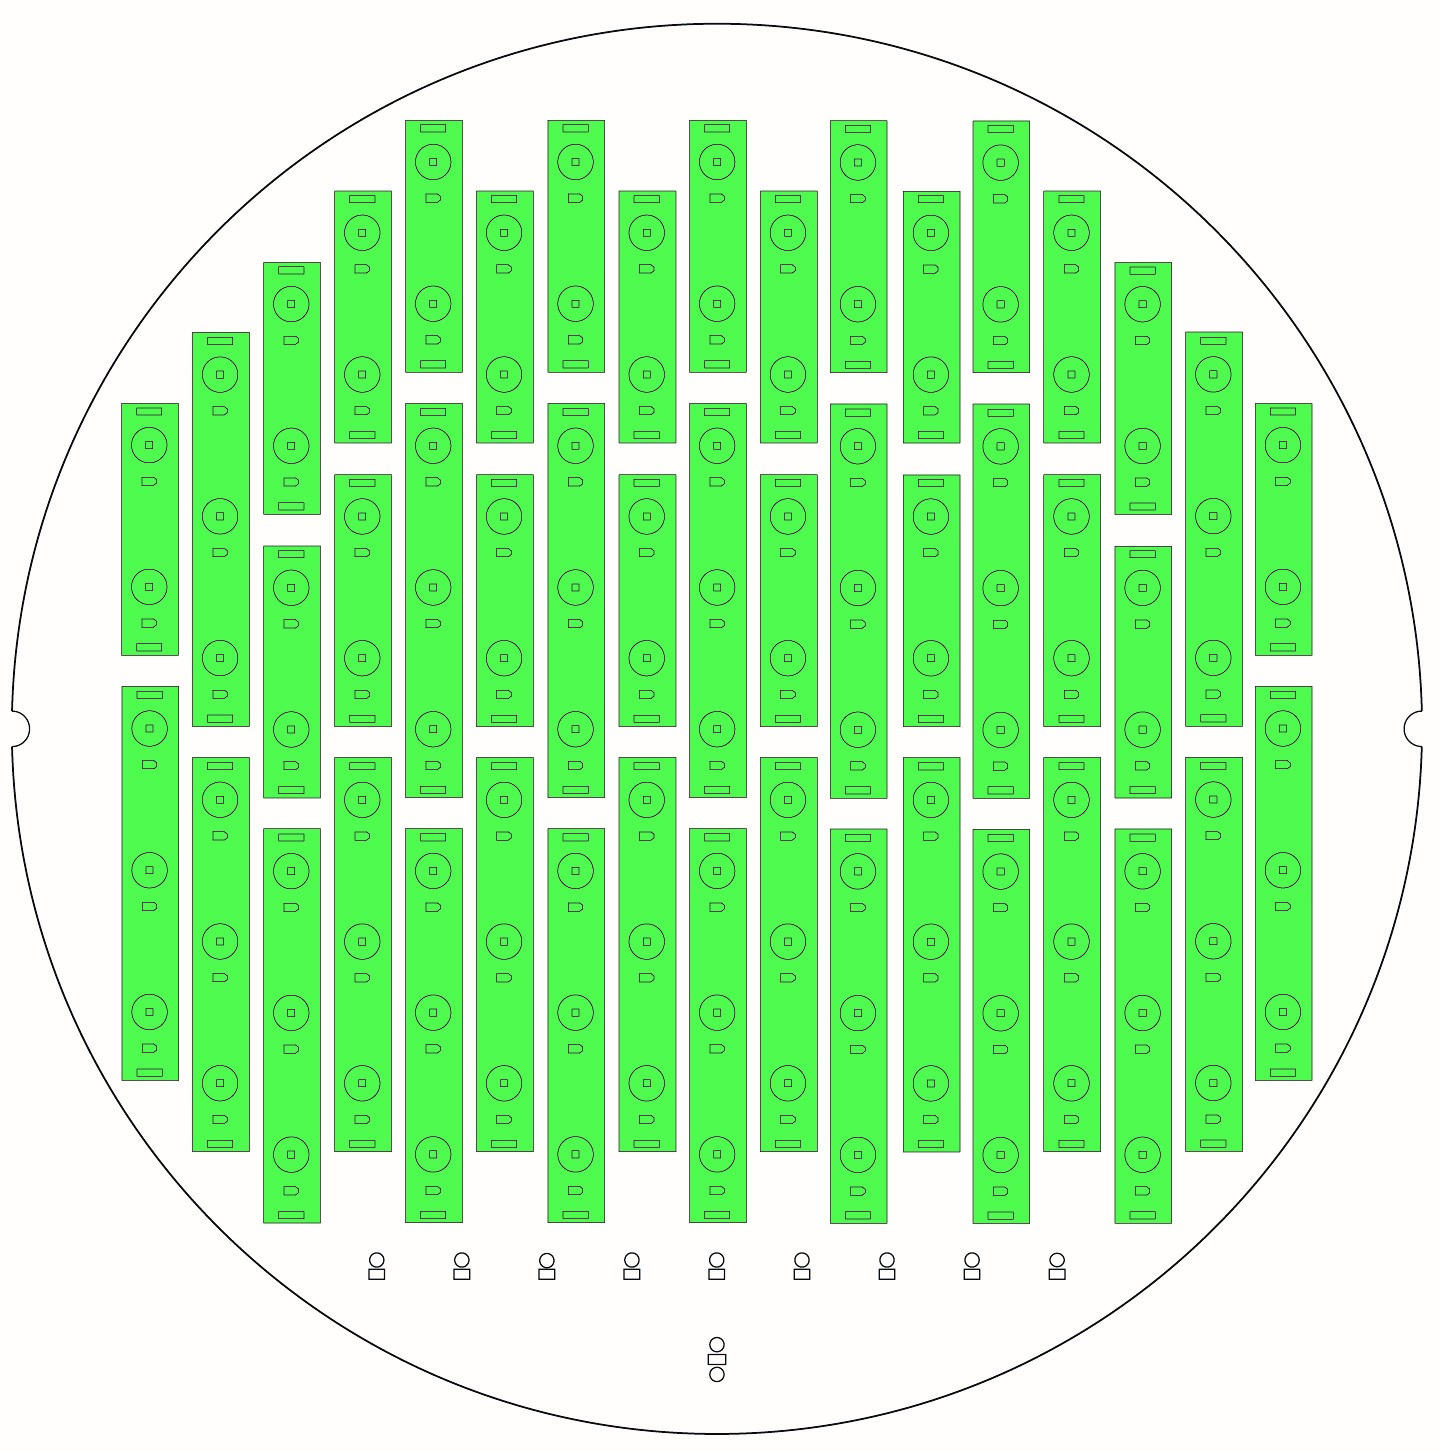
\includegraphics[width=0.7\textwidth]{./dados/figuras/placas-matriz-colunas}
    \fonte{adaptado de (MITSUKO, 2016)}
    \label{fig:placas-matriz-colunas}
\end{figure}

Uma vez definido que a matriz seria composta por placas com 2 ou 3 bolinhas, iniciaram-se os testes de conceito com o protótipo, apresentado na \autoref{fig:matriz-prototipo}. Nesses ensaios, foram testados os conceitos de endereçamento do LED WS2812, a leitura do nível lógico dos sensores através dos registradores de deslocamento e também o modo de conexão entre as placas.

\begin{figure}[H]
    \centering
    \caption{Protótipo das placas da matriz}
    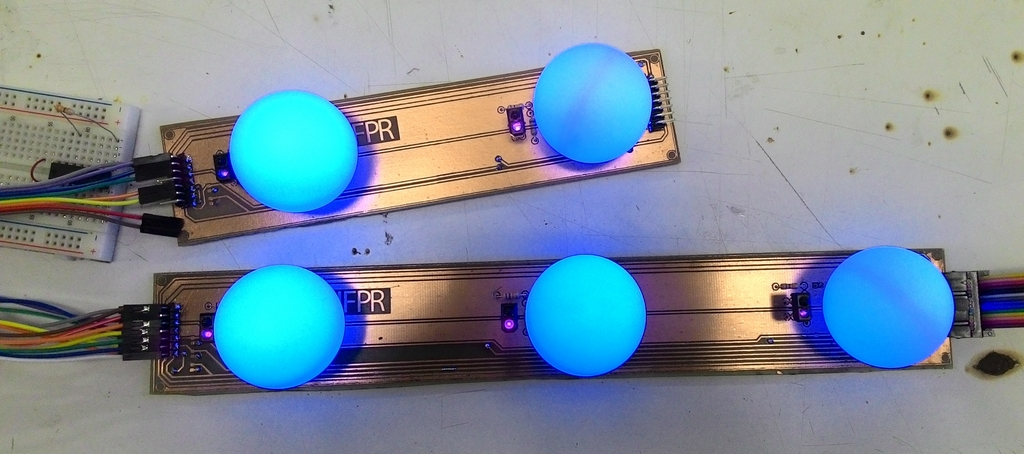
\includegraphics[width=0.8\textwidth]{./dados/figuras/mesa-protoboard}
    \fonte{(O AUTOR, 2017)}
    \label{fig:matriz-prototipo}
\end{figure}

Todos os conceitos propostos foram validados e as 47 placas que compõem a matriz foram confeccionadas em produção industrial. A \autoref{fig:placa2} e a \autoref{fig:placa3} apresentam as faces superior e inferior dos módulos.

\begin{figure}[H]
    \centering
    \caption{Faces da PCI do módulo de 2 bolinhas}
    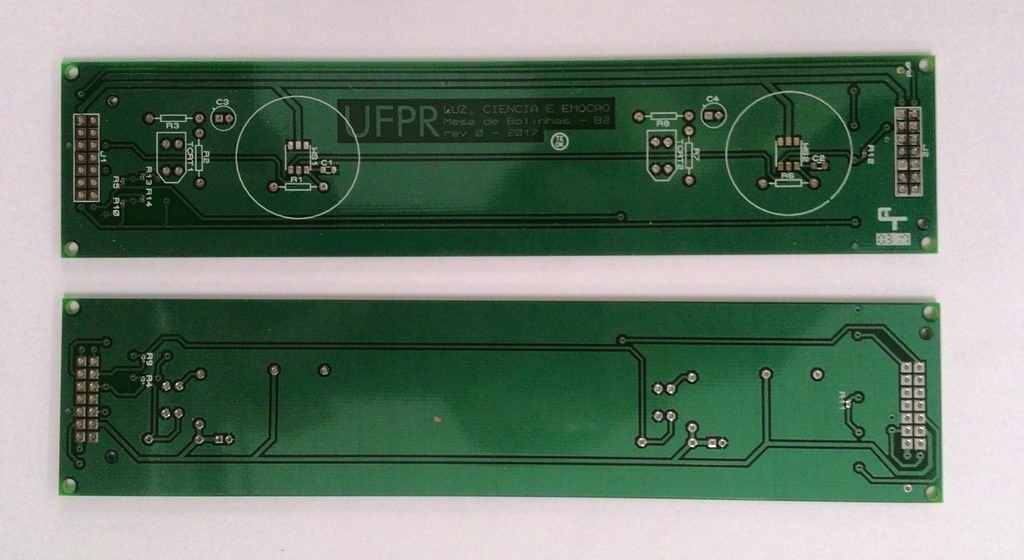
\includegraphics[width=0.8\textwidth]{./dados/figuras/bloco-2}
    \fonte{(O AUTOR, 2017)}
    \label{fig:placa2}
\end{figure}

\begin{figure}[H]
    \centering
    \caption{Faces da PCI do módulo de 3 bolinhas}
    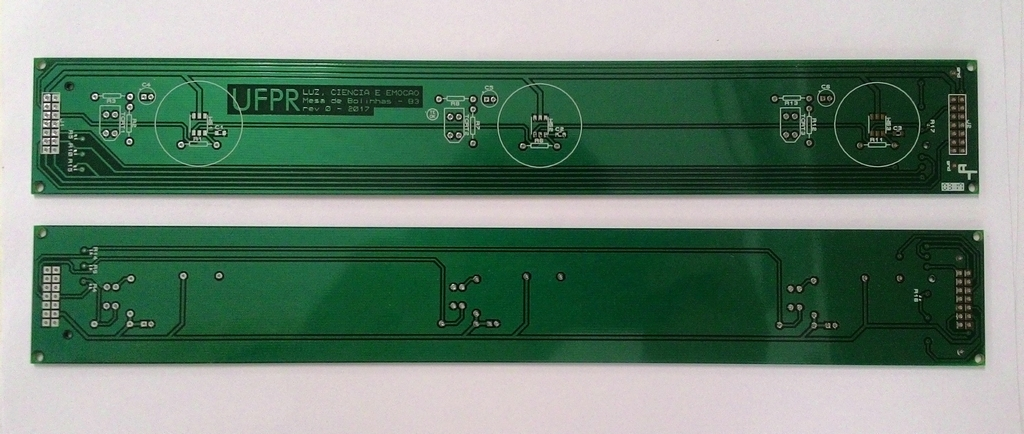
\includegraphics[width=0.99\textwidth]{./dados/figuras/bloco-3}
    \fonte{(O AUTOR, 2017)}
    \label{fig:placa3}
\end{figure}

\textcolor{red}{TODO: o ``resultado da matriz fica nesta seção mesmo?''}

\section{PROJETO DA INTERFACE}
\label{sec:interface}

Como já brevemente introduzido pela \autoref{sec:concepcao} (Concepção do Projeto), a Interface tem a função de interligar as seções Matriz e Controlador. Contudo, deve-se atentar a algumas questões:

\begin{enumerate}[label=\Roman*.]
    \item Tanto o barramento dos sensores, quanto o barramento dos LEDs devem seguir a sequência da esquerda para a direita; de baixo para cima;
    \item Por integrar barramentos de frequências razoáveis - NRZ @800kHz e SPI @4MHz dos LEDs e sensores, respectivamente - deve-se evitar construir trilhas com quinas abruptas, em função da reflexão do sinal;
    %\item As trilhas de potência devem ser adequadas para suportarem a corrente no caso mais extremo.
\end{enumerate}

A questão (I) foi trabalhada visando a redução de custo, decidiu-se que Interface também seria um projeto modular, isto é, esta seção seria dividida em placas do mesmo modelo. Isso é em razão do valor das placas de circuito impresso ser calculado em função de sua área e que cada projeto possui um pedido mínimo. Em outras palavras, quanto maior a área de uma PCI, maior será o seu custo, e quanto mais modelos de placa, maior será a quantidade a ser adquirida, pois cada modelo possui um pedido mínimo para produção. Sendo assim, a Interface foi projetada para abranger todas as colunas da Matriz em duas ``metades'', como é apresentado na \autoref{fig:colunas}. No caso, uma placa teria a função de operar as primeiras 9 colunas (de A a I) e a outra, as 8 colunas restantes (de J a Q).

\begin{figure}[H]
    \centering
    \caption{Divisão das colunas para conexão com a Interface}
    \includegraphics[width=0.7\textwidth]{./dados/figuras/colunas}
    \fonte{adaptado de (MITSUKO, 2016)}
    \label{fig:colunas}
\end{figure}

A \autoref{fig:diagrama-interface} apresenta o diagrama da formação do barramento dos sensores. Nele, cada coluna da Matriz é conectada a um registrador de deslocamento, em forma sequencial (A:1, ..., I:9; J:1, ..., Q:8). Nota-se também que o último registrador da segunda placa não possui conexão, dado que todas as colunas já foram abrangidas registradores precedentes.

\begin{figure}[H]
    \centering
    \caption{Diagrama do barramento da Interface}
    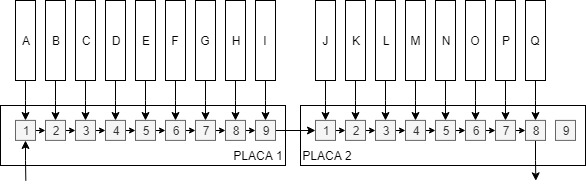
\includegraphics[width=0.75\textwidth]{./dados/figuras/interface}
    \fonte{(O AUTOR, 2018)}
    \label{fig:diagrama-interface}
\end{figure}

Esse direcionamento do barramento é dado por um resistor de $0\Omega$, como apresentado na \autoref{fig:direcionamento-shift} (componente ``R2''). Se montado, o sinal é diretamente conduzido ao conector de saída (``P11''), ignorando o último registrador (``U9'') que, neste caso, não seria montado.

\begin{figure}[H]
    \centering
    \caption{Direcionamento do barramento dos sensores}
    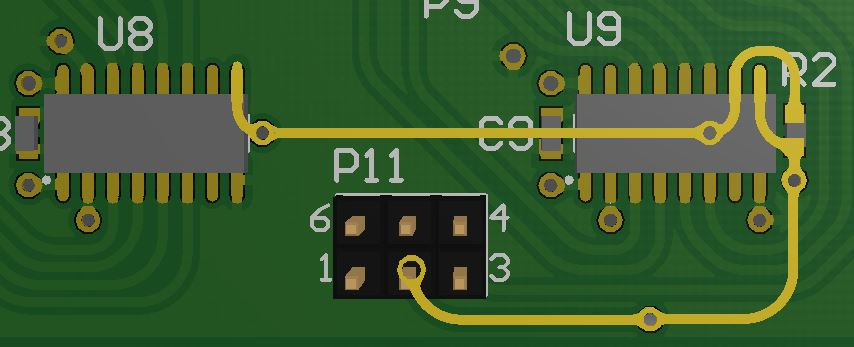
\includegraphics[width=0.6\textwidth]{./dados/figuras/res-dir-shift}
    \fonte{(O AUTOR, 2018)}
    \label{fig:direcionamento-shift}
\end{figure}

De iguais modos, o barramento dos LEDs foi projetado para seguir a mesma sequência (\autoref{fig:sentido-leds}) e o direcionamento entre a última coluna (``P9'') ou o conector de saída (``P11'') também é dado através de um resistor de $0\Omega$ (``R1''), como apresentado na \autoref{fig:direcionamento-leds}.

\begin{figure}[H]
    \centering
    \caption{Sentido do barramento dos LEDs}
    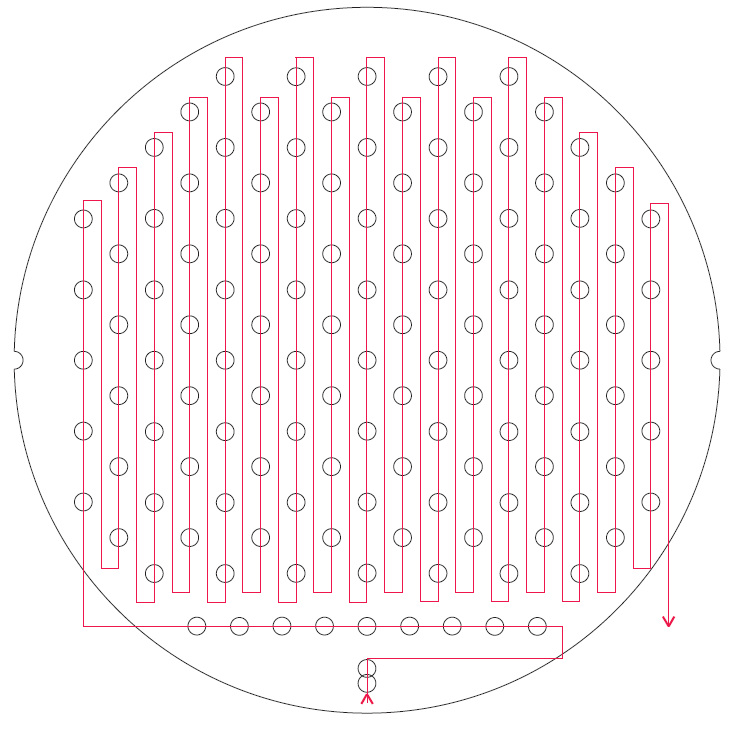
\includegraphics[width=0.75\textwidth]{./dados/figuras/sentido-leds}
    \fonte{adaptado de (MITSUKO, 2016)}
    \label{fig:sentido-leds}
\end{figure}

\begin{figure}[H]
    \centering
    \caption{Direcionamento do barramento dos LEDs}
    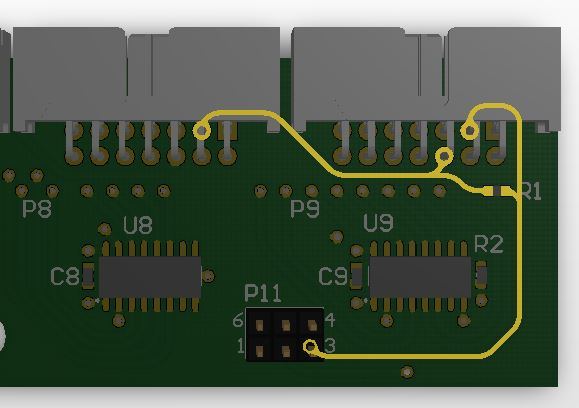
\includegraphics[width=0.6\textwidth]{./dados/figuras/dir-leds}
    \fonte{(O AUTOR, 2018)}
    \label{fig:direcionamento-leds}
\end{figure}

Já em relação à questão (II), sobre a possibilidade de reflexão de sinais devido à perturbação da capacitância e auto-indutância da trilha, seguiu-se a recomendação de leiaute de \cite{datasheet-ti}, apresentada na \autoref{fig:leiaute-ti}.

\begin{figure}[H]
    \centering
    \caption{Recomendação de leiaute para as trilhas de sinal}
    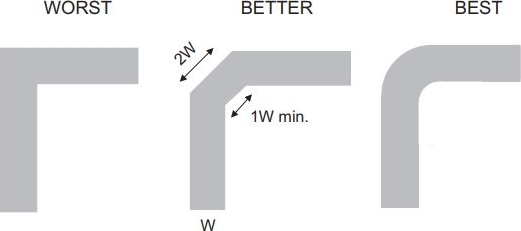
\includegraphics[width=0.5\textwidth]{./dados/figuras/leiaute-ti}
    \fonte{\citeonline{datasheet-ti}}
    \label{fig:leiaute-ti}
\end{figure}

Tal técnica foi aplicada não só nas trilhas de sinais, mas também em todas as ocasiões possíveis, como apresentado na \autoref{fig:trilhas-arredondadas}.

\begin{figure}[H]
    \centering
    \caption{Trilhas arredondadas}
    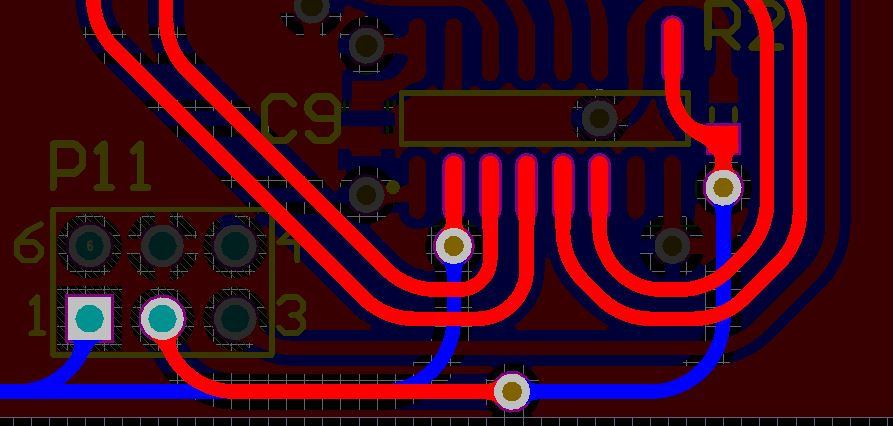
\includegraphics[width=0.7\textwidth]{./dados/figuras/trilhas-arredondadas}
    \fonte{(O AUTOR, 2018)}
    \label{fig:trilhas-arredondadas}
\end{figure}

Além disso, para evitar a propagação do ruído da parte de potência, a alimentação do circuito lógico (``VCC5V'') foi separada da alimentação dos LEDs (``VLED'') e da dos sensores (``VSENSOR''), conforme apresentado na \autoref{fig:interface-alimentacao}. Ademais, a conexão física entre as massas (terra) é feita somente em um único ponto, assim, o retorno da alimentação de potência ("GND\_MATRIX") permanece confinado, não circulando sobre o plano de terra ("GND"). Essa técnica é conhecida por \emph{``net-tie''} e está destacada na \autoref{fig:interface-nettie}.

\begin{figure}[H]
    \centering
    \caption{Separação das alimentações da Interface}
    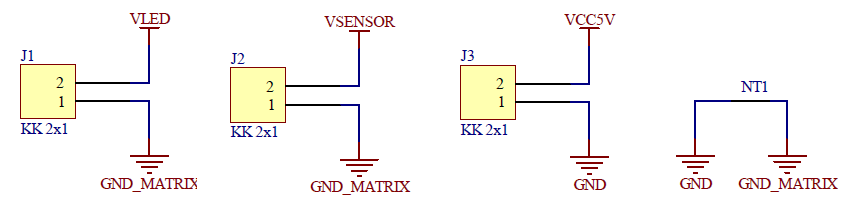
\includegraphics[width=0.85\textwidth]{./dados/figuras/alimentacao-interface}
    \fonte{(O AUTOR, 2018)}
    \label{fig:interface-alimentacao}
\end{figure}

\begin{figure}[H]
    \centering
    \caption{Separação física das massas}
    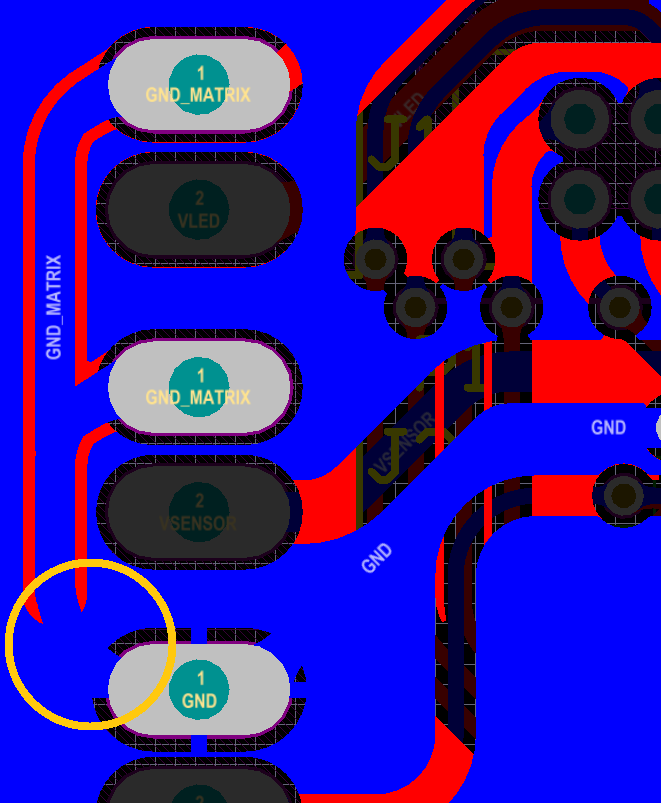
\includegraphics[width=0.4\textwidth]{./dados/figuras/nt-interface}
    \fonte{(O AUTOR, 2018)}
    \label{fig:interface-nettie}
\end{figure}

Por fim, a \autoref{fig:3d-interface} apresenta o modelo 3D da placa de interface. Trata-se de uma PCI face-dupla, 245mm x 32,76mm. Os conectores de alimentação (à esquerda da placa) são da série KK Molex\textsuperscript{\textregistered}, que impedem a inversão de polaridade na conexão com fonte de alimentação externa, e os conectores das colunas (parte superior da placa) são do padrão \emph{Latch-header}, recomendado para aplicações com limitação de espaço. Cada placa suporta até 9 colunas de até 8 sensores, e as PCIs podem ser ligadas em série para compartilharem o mesmo barramento.

\begin{figure}[H]
    \centering
    \caption{Modelo 3D da Interface}
    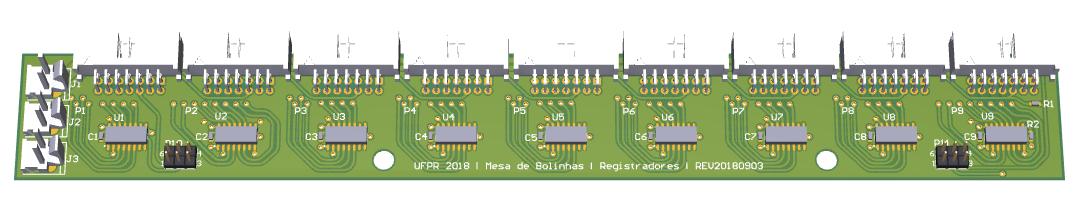
\includegraphics[width=1.0\textwidth]{./dados/figuras/interface-3d}
    \fonte{(O AUTOR, 2018)}
    \label{fig:3d-interface}
\end{figure}

\section{PROJETO DO CONTROLADOR}
\label{sec:controlador}

O Controlador é responsável por comandar os eventos de interação, através da Interface, da seção Matriz. Ademais, engloba também o seletor de cores, circuito de gravação, teclado para depuração e suporte para um barramento externo. A \autoref{fig:diagrama-controlador} apresenta seu diagrama simplificado.

\begin{figure}[H]
    \centering
    \caption{Diagrama da seção Controlador}
    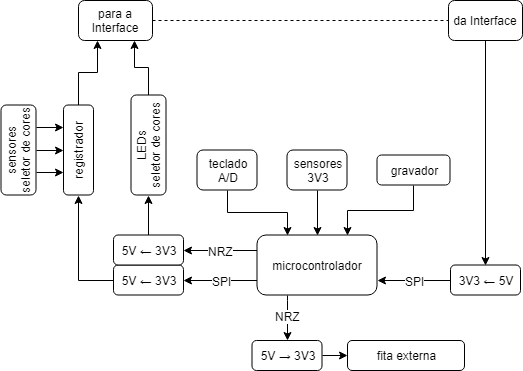
\includegraphics[width=0.75\textwidth]{./dados/figuras/diagrama-controlador}
    \fonte{(O AUTOR, 2018)}
    \label{fig:diagrama-controlador}
\end{figure}

\subsection{ALIMENTAÇÃO  E CONVERSÃO DE NÍVEL LÓGICO}
\label{subsec:alimentacao}

Da mesma forma que na Interface, a alimentação do Controlador também foi dividida, separando os circuitos de potência (``VLED'') e lógico (``VCC5V''), inclusive com \emph{net-tie} isolando fisicamente as massas. Porém, diferente da Matriz, onde a quantidade de LEDs e sensores é muito maior que a do seletor de cores do Controlador, esses circuitos compartilham a mesma alimentação de potência neste projeto. A \autoref{fig:alimentacao-controlador} apresenta o circuito de entrada de alimentação.

Como o microcontrolador operar em 3,3V, houve a necessidade de incluir um regulador para a faixa especificada. Por se tratar de um circuito de carga simples, isto é, de baixo consumo, optou-se por um regulador linear de saída fixa (componente ``U2''). Para protegê-lo da descarga das capacitâncias conectadas à sua saída (por exemplo, o capacitor ``C23''), foi incluído um diodo de \emph{bypass} (``D27'') para desviar a corrente reversa sobre regulador, no caso da fonte externa ser desconectada e a tensão de saída resultar em um potencial mais alto que o de entrada. Esse diodo também possui a função de proteger o regulador caso o desenvolvedor queira alimentar a placa diretamente através do circuito de gravação, a ser discutido mais adiante.

\begin{figure}[H]
    \centering
    \caption{Entrada de alimentação do Controlador}
    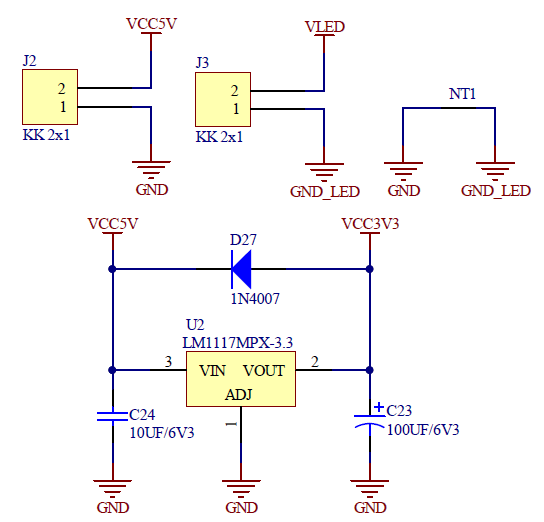
\includegraphics[width=0.7\textwidth]{./dados/figuras/alimentacao-controlador}
    \fonte{(O AUTOR, 2018)}
    \label{fig:alimentacao-controlador}
\end{figure}

\subsection{SELETOR DE CORES}
\label{subse:seletor}

O seletor de cores forma a primeira etapa dos barramentos, seja dos LEDs endereçáveis ou dos registradores de deslocamento. É composto por 10 sensores reflexivos e 11 LEDs endereçáveis, como apresentado na \autoref{fig:seletor-cores}, e a \autoref{fig:diagrama-seletor-cores} apresenta seu diagrama.

\begin{figure}[H]
    \centering
    \caption{Vista do seletor de cores}
    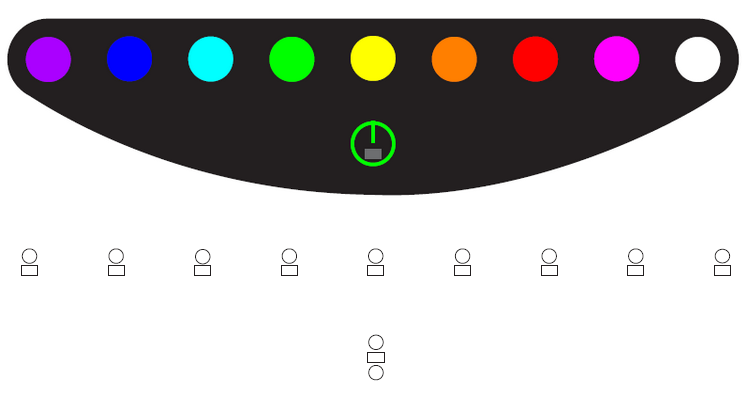
\includegraphics[width=0.75\textwidth]{./dados/figuras/seletor-cores}
    \fonte{adaptado de (MITSUKO, 2016)}
    \label{fig:seletor-cores}
\end{figure}

\begin{figure}[H]
    \centering
    \caption{Vista do seletor de cores}
    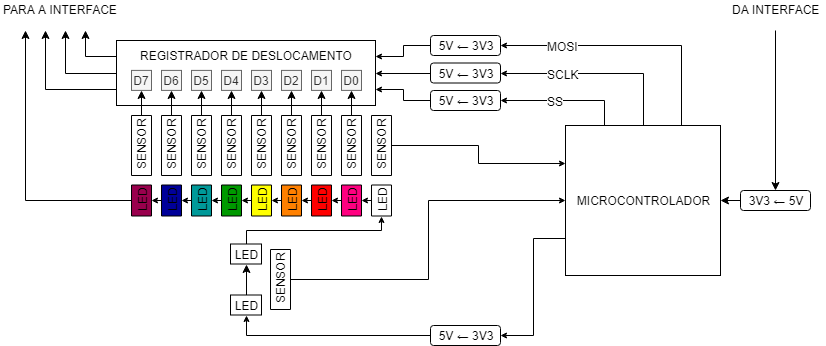
\includegraphics[width=0.99\textwidth]{./dados/figuras/diagrama-seletor-cores}
    \fonte{(O AUTOR, 2018)}
    \label{fig:diagrama-seletor-cores}
\end{figure}

Assim como feito com as colunas da Matriz, por meio das placas da Interface, o registrador de deslocamento é responsável por coletar os níveis lógicos de 8 dos 10 sensores do seletor de cores, restando 2 sensores fora do barramento. Assim, optou-se por conectá-los diretamente aos pinos do microcontrolador, visto que haviam GPIOs livres.

Devido aos LEDs e registradores de deslocamento serem alimentados em 5V, enquanto que o microcontrolador é alimentado em 3,3V, foi necessário adequar os sinais dos barramentos através de conversores de nível lógico. Essa conversão se deu de duas formas, nos seguintes sinais:

\begin{itemize}
    \item De 3,3V para 5V:
        \begin{itemize}
            \item Saída de dados do barramento NRZ (LEDs WS2812)
            \item Saída de dados do barramento SPI (MOSI)
            \item Saída de clock do barramento SPI (SCLK)
            \item Sinal de seleção de periférico do barramento SPI (SS)
        \end{itemize}
    \item De 5V para 3,3V:
        \begin{itemize}
            \item Entrada de dados do barramento SPI (MISO)
        \end{itemize}
\end{itemize}

Os conversores de nível de 3,3V para 5V foram projetados na topologia não-inversora, com transistor NPN operando nas regiões de corte e saturação: mantêm-se base e coletor polarizados - base em 3,3V e coletor em 5V - enquanto que a polarização da junção base-emissor ($V_{BE}$) é dada pela aplicação do sinal no emissor.

A \autoref{fig:3v3-5v} apresenta o esquemático do conversor para o sinal de \emph{clock} do barramento SPI. Nota-se que, quando o sinal ``ESP\_CLOCK'' (saída SCLK do microcontrolador ESP8266) vai a 1-lógico (3,3V), não há diferença de potencial entre a base e o emissor ($V_{BE}=0V$), portanto, o transistor está em corte, logo a saída ``SHIFT\_CLK'' (entrada de \emph{clock} do \emph{shift-register}) vai a 5V (1-lógico).

No caso da aplicação de 0V (0-lógico) por ``ESP\_CLOCK'', a junção base-emissor estará diretamente polarizada, o que, neste caso, levará o transistor à saturação. Com isso, a tensão em ``SHIFT\_CLK'' será a diferença de potencial entre coletor e emissor ($V_{CE}$) somada à queda de tensão sobre o \emph{mosfet} interno da GPIO do microcontrolador, resultando em um potencial relativamente próximo a 0V (0-lógico).

Cabe aqui ressaltar inclusão do diodo de \emph{Baker clamping} para minimizar os efeitos das capacitâncias parasitas do transistor.

\begin{figure}[H]
    \centering
    \caption{Conversor de nível lógico da linha de \emph{clock} do barramento SPI}
    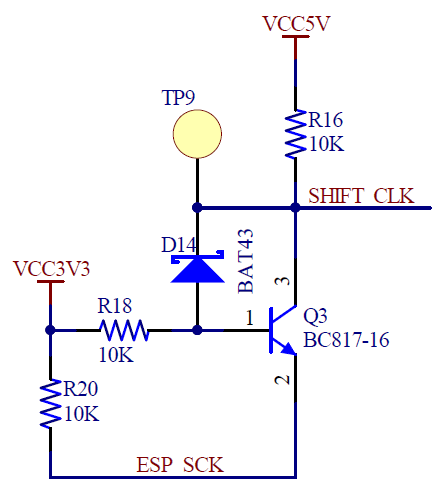
\includegraphics[width=0.4\textwidth]{./dados/figuras/3v3-5v}
    \fonte{(O AUTOR, 2018)}
    \label{fig:3v3-5v}
\end{figure}

Já para a situação de transformação de 5V para 3,3V, como é o caso do retorno do sinal dos registradores de deslocamento das placas de interface (sinal MISO), a implementação do conversor de nível lógico foi dada por um simples divisor resistivo, como apresentado na \autoref{fig:5v-3v3}.

\begin{figure}[H]
    \centering
    \caption{Conversor de nível lógico da linha MISO do barramento SPI}
    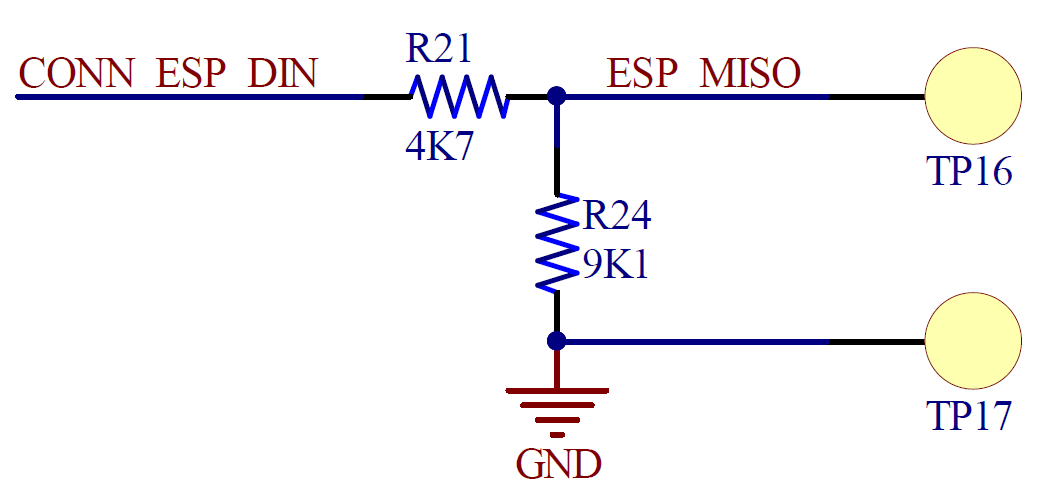
\includegraphics[width=0.5\textwidth]{./dados/figuras/5v-3v3}
    \fonte{(O AUTOR, 2018)}
    \label{fig:5v-3v3}
\end{figure}

Quando aplicado 5V (1-lógico) em ``CONN\_ESP\_DIN'' (entrada de dados do conector, linha MISO do barramento SPI), a tensão em ``ESP\_MISO'' (linha MISO do microcontrolador) será aproximadamente 3,3V (1-lógico), dado pela \autoref{eq:5v-3v3}. De mesmo modo, quando aplicado 0V na entrada do conversor, não haverá queda de tensão sobre o resistor de saída (''`R24``), portanto a tensão em ``ESP\_MISO'' também será 0V (0-lógico).

\begin{equation}
    V = 5V \cdot \frac{9100\Omega}{9100\Omega+4700\Omega} = 3,297V
    \label{eq:5v-3v3}
\end{equation}

\subsection{GRAVADOR}
\label{subsec:gravador}

O microcontrolador ESP8266 possui alguns modos de operação, entre eles, o modo normal e o de gravação via UART, que são determinados pelo estado de alguns pinos durante a inicialização do sistema (\emph{boot}), como brevemente introduzido na \autoref{sec:microcontrolador}.

Além de fornecer uma via para a comunicação serial com um adaptador USB, o circuito apresentado a seguir (\autoref{fig:circuito-gravador}) também tem a função de forçar o microcontrolador a entrar em modo de gravação conforme os comandos de \emph{``reset''} e \emph{``data terminal ready''} (DTR) do adaptador. Dessa forma, não há a necessidade de uma operação manual para determinar os estados dos pinos de programação para carregar um novo \emph{firmware} no microcontrolador. Para tal, basta somente que o adaptador disponha de uma linha DTR, como o exemplo apresentado na \autoref{fig:ftdi}. Cabe aqui ressaltar que, assim como citado na \autoref{subsec:alimentacao}, todo o circuito de 3,3V pode ser alimentado diretamente pelo adaptador USB (desde que seja 3,3V), sem a necessidade de uma fonte externa. Isso simplifica o desenvolvimento e a depuração do projeto, quando não houver a necessidade de testar o restante do circuito.

\begin{figure}[H]
    \centering
    \caption{Exemplo de adaptador serial-USB com linha DTR}
    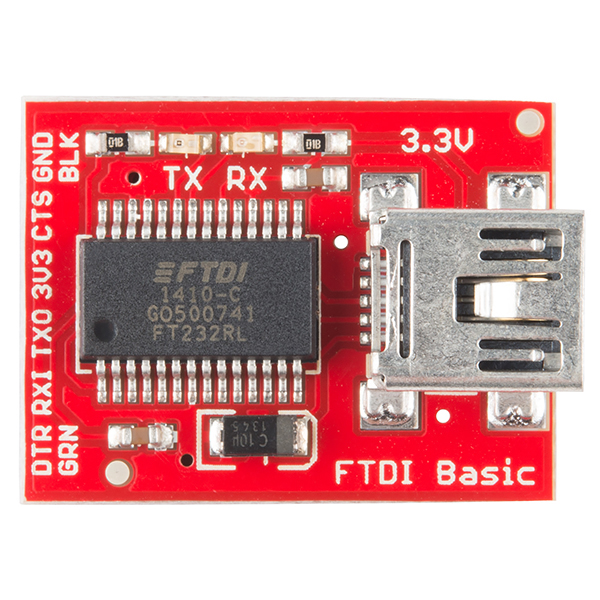
\includegraphics[width=0.3\textwidth]{./dados/figuras/ftdi}
    \fonte{\citeonline{adaptador-usb}}
    \label{fig:ftdi}
\end{figure}

Sobretudo, para que o microcontrolador entre em modo de gravação, o pino ``GPIO 0'' deve estar em 0-lógico durante a inicialização. Se estiver em 1-lógico durante o \emph{reset}, o ESP8266 inicializa em modo normal, executando o programa armazenado na memória interna.

\begin{figure}[H]
    \centering
    \caption{Esquemático do circuito de gravação}
    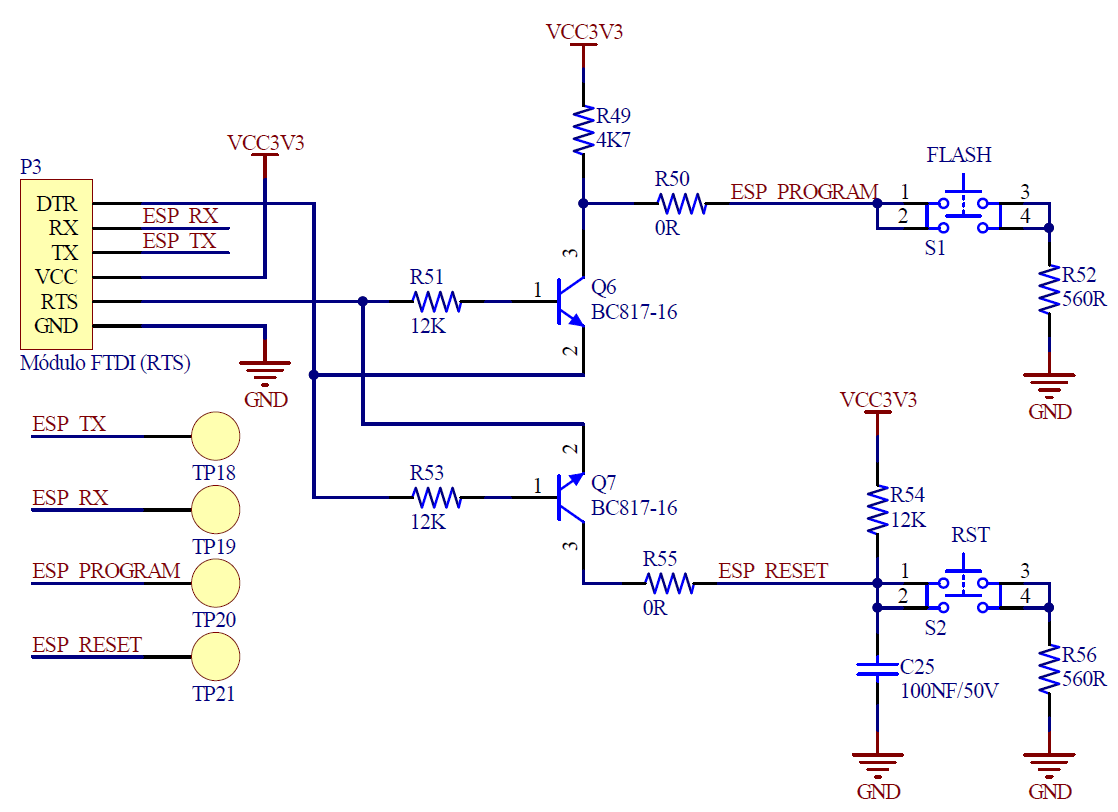
\includegraphics[width=0.8\textwidth]{./dados/figuras/gravacao}
    \fonte{(O AUTOR, 2018)}
    \label{fig:circuito-gravador}
\end{figure}

A \autoref{tab:gravador} apresenta os estados dos pinos do microcontrolador em função dos níveis do adaptador USB, através do circuito da \autoref{fig:circuito-gravador}. Nota-se que a condição de gravação (GPIO 0 = zero lógico) é dada somente \textcolor{red}{TODO: .......... ????}.

\begin{table}[H]
    \centering
    \caption[Tabela verdade do gravador automático]{Tabela verdade do gravador automático.
    \label{tab:gravador}}
\begin{tabular}{|c|c|c|c|}
\hline
\multicolumn{2}{|c|}{\textbf{Adaptador USB}} & \multicolumn{2}{c|}{\textbf{ESP8266}} \\ \hline
\textbf{DTR} & \textbf{RST} & \textbf{GPIO 0} & \textbf{Reset} \\ \hline
0 & 0 & 1 & 1 \\ \hline
0 & 1 & 0 & 1 \\ \hline
1 & 0 & 1 & 0 \\ \hline
1 & 1 & 1 & 1 \\ \hline
\end{tabular}
    \fonte{(O AUTOR, 2018)}
\end{table}


Contudo, se o desenvolvedor não dispor de um adaptador USB com sinal DTR, ainda há a possibilidade de pôr o microcontrolador em modo de gravação de maneira manual, através dos botões ``S1'' e ``S2''.

\subsection{TECLADO AD}
\label{subsec:tecladoad}

O ``Teclado AD'' (ou teclado analógico) tem a função de servir como interface durante as etapas de desenvolvimento/depuração. Com apenas um único pino do microcontrolador é possível ler diversas teclas, desde que seja um pino com função Conversor Analógico-Digital. A \autoref{fig:tecladoad} apresenta o esquemático do circuito.

\begin{figure}[H]
    \centering
    \caption{Esquemático do circuito do teclado analógico}
    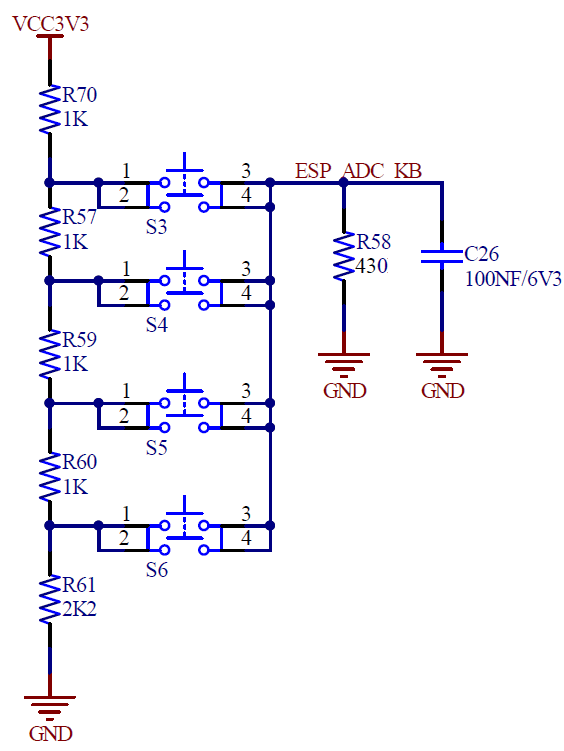
\includegraphics[width=0.5\textwidth]{./dados/figuras/tecladoad}
    \fonte{(O AUTOR, 2018)}
    \label{fig:tecladoad}
\end{figure}

Seu funcionamento se dá por meio da combinação de uma cadeia de resistores. Através da Lei de Ohm, pelas combinações série-paralelo, é possível estimar qual botão está sendo pressionado, limitando-se a um botão por vez.

A \autoref{tab:tecladoad} apresenta os valores de tensão e as unidades estimadas pelo conversor interno do microcontrolador, um ADC de 10 \emph{bits} de resolução, com faixa de operação de 0V a 1V.

\begin{table}[H]
    \centering
    \caption[Valores de tensão e unidades do teclado analógico]{Valores de tensão e unidades do teclado analógico.
    \label{tab:tecladoad}}
\begin{tabular}{|c|c|c|}
\hline
\textbf{Chave} & \textbf{Tensão (V)} & \textbf{Valor ADC} \\ \hline
\textbf{S3} & 0,94 & 960 \\ \hline
\textbf{S4} & 0,54 & 551 \\ \hline
\textbf{S5} & 0,37 & 379 \\ \hline
\textbf{S6} & 0,27 & 279 \\ \hline
\end{tabular}
    \fonte{(O AUTOR, 2018)}
\end{table}


\subsection{PROJETO DA PCI DO CONTROLADOR}
\label{subsec:pcicontrol}

Em sua totalidade, não há um padrão de repetição de funcionalidades como nos outros setores (Interface e Matriz), então a placa do Controlador não foi projetada de maneira modular, senão em placa única que, inclusive, resultou em uma PCI relativamente grande (), a ser discutida na \autoref{chap:}.A \autoref{fig:controlador-top} apresenta a visão da face superior do modelo 3D da placa, e a \autoref{fig:controlador-bottom} apresenta a visão da face inferior.

\begin{figure}[H]
    \centering
    \caption{Visão superior do modelo 3D da placa do Controlador}
    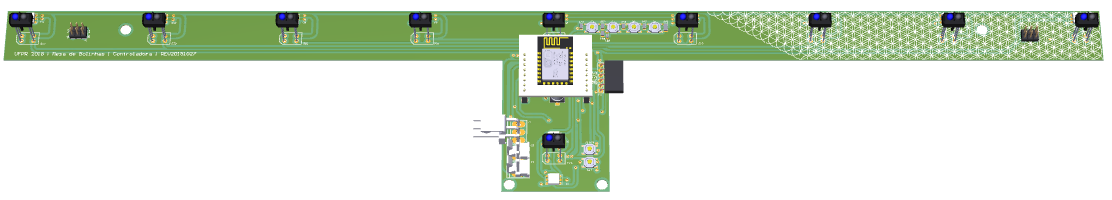
\includegraphics[width=1.0\textwidth]{./dados/figuras/controlador-top}
    \fonte{(O AUTOR, 2018)}
    \label{fig:controlador-top}
\end{figure}

\begin{figure}[H]
    \centering
    \caption{Visão inferior do modelo 3D da placa do Controlador}
    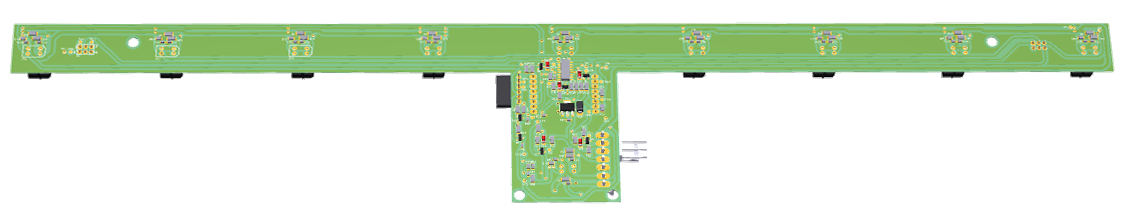
\includegraphics[width=1.0\textwidth]{./dados/figuras/controlador-bottom}
    \fonte{(O AUTOR, 2018)}
    \label{fig:controlador-bottom}
\end{figure}

Assim como nos projetos anteriores, a placa do Controlador também foi projetada utilizando-se de técnicas para evitar a reflexão dos sinais, separação das alimentações dos circuitos de potência e utilização de conectores que impedem inversão de polaridade. Além disso, com exceção dos sensores e conectores, todos os componentes são de montagem em superfície (SMD), como apresentado na \autoref{fig:controlador-smd}.

\begin{figure}[H]
    \centering
    \caption{Visão inferior do modelo 3D da placa do Controlador - detalhe para os componentes SMDs}
    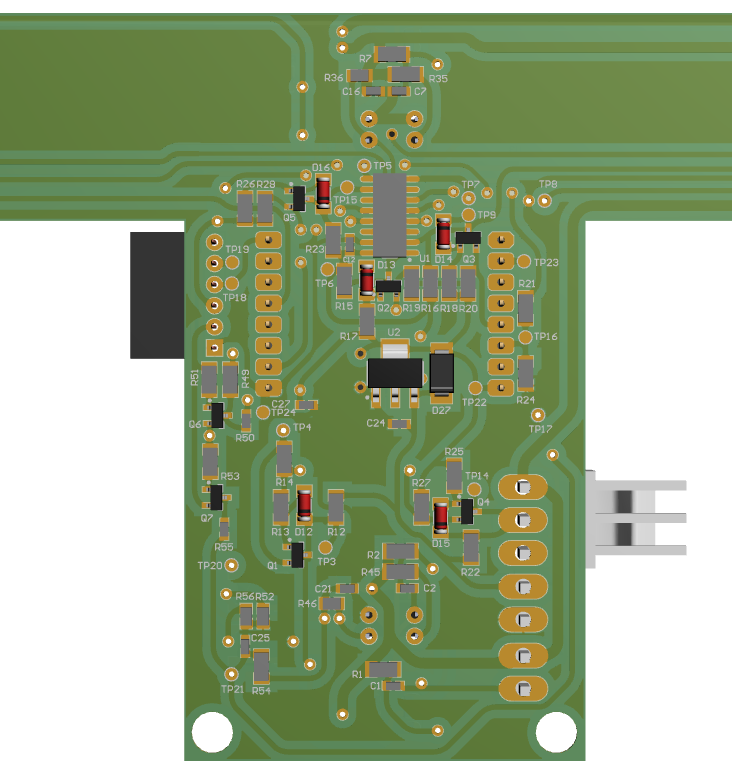
\includegraphics[width=0.7\textwidth]{./dados/figuras/controlador-smd}
    \fonte{(O AUTOR, 2018)}
    \label{fig:controlador-smd}
\end{figure}

\section{PROJETO DO \emph{FIRMWARE}}
\label{sec:firmware}

\subsection{\emph{DEBOUNCE}}
\label{subsec:debounce}

\subsection{MÁQUINA DE ESTADOS FINITA}
\label{subsec:fsm}

\textcolor{red}{TODO: citar a referencia gang  of 4}

                   % Metodologia
% RESULTADOS-------------------------------------------------------------------

\chapter{ANÁLISE E DISCUSSÃO DOS RESULTADOS}

Cada capítulo deve conter uma pequena introdução (tipicamente, um ou dois parágrafos) que deve deixar claro o objetivo e o que será discutido no capítulo, bem como a organização do capítulo.
                    % Resultados
%% ORIENTAÇÕES GERAIS------------------------------------------------------------


% SOBRE AS ILUSTRAÇÕES----------------------------------------------------------
\chapter{SOBRE AS ILUSTRAÇÕES}
\label{chap:apSobreIlust}

A seguir exemplifica-se como inserir ilustrações no corpo do trabalho. As ilustrações serão indexadas automaticamente em suas respectivas listas. A numeração sequencial de figuras, tabelas e equações também ocorre de modo automático.

Referências cruzadas são obtidas através dos comandos \verb|\label{}| e \verb|\ref{}|. Sendo assim, não é necessário por exemplo, saber que o número de certo capítulo é \ref{chap:fundamentacaoTeorica} para colocar o seu número no texto. Outra forma que pode ser utilizada é esta: \autoref{chap:fundamentacaoTeorica}, facilitando a inserção, remoção e manejo de elementos numerados no texto sem a necessidade de renumerar todos esses elementos.

% FIGURAS-----------------------------------------------------------------------
\chapter{FIGURAS}
\label{chap:figuras}

Exemplo de como inserir uma figura. A \autoref{fig:figura-exemplo1} aparece automaticamente na lista de figuras. Para saber mais sobre o uso de imagens no \LaTeX{} consulte literatura especializada \cite{Goossens2007}.

Os arquivos das figuras devem ser armazenados no diretório de "/dados".

\begin{figure}[!htb]
    \centering
    \caption{Exemplo de Figura}
    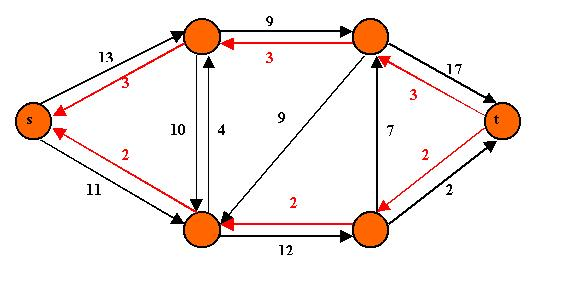
\includegraphics[width=0.5\textwidth]{./dados/figuras/figura1}
    \fonte{\citeonline{IRL2014}}
    \label{fig:figura-exemplo1}
\end{figure}

% QUADROS E TABELAS---------------------------------------------------------------
\chapter{QUADROS E TABELAS}
\label{chap:tabelas}

Exemplo de como inserir o \autoref{qua:quadro-exemplo1} e a \autoref{tab:tabela-exemplo1}. Ambos aparecem automaticamente nas suas respectivas listas. Para saber mais informações sobre a construção de tabelas no \LaTeX{} consulte literatura especializada \cite{Mittelbach2004}.

Ambos os elementos (Quadros e Tabelas) devem ser criados em arquivos separados para facilitar manutenção e armazenados no diretório de "/dados".

\begin{quadro}[!htb]
    \centering
    \caption{Exemplo de Quadro.\label{qua:quadro-exemplo1}}
    \begin{tabular}{|p{7cm}|p{7cm}|}
        \hline
        \textbf{BD Relacionais} & \textbf{BD Orientados a Objetos} \\
        \hline
        Os dados são passivos, ou seja, certas operações limitadas podem ser automaticamente acionadas quando os dados são usados. Os dados são ativos, ou seja, as solicitações fazem com que os objetos executem seus métodos. & Os processos que usam dados mudam constantemente. \\
        \hline
    \end{tabular}
    \fonte{\citeonline{Barbosa2004}}
\end{quadro}


A diferença entre quadro e tabela está no fato que um quadro é formado por linhas horizontais e verticais. Deve ser utilizado quando o conteúdo é majoritariamente não-numérico. O número do quadro e o título vem acima do quadro, e a fonte, deve vir abaixo. E Uma tabela é formada apenas por linhas verticais. Deve ser utilizada quando o conteúdo é majoritariamente numérico. O número da tabela e o título vem acima da tabela, e a fonte, deve vir abaixo, tal como no quadro.

\begin{table}[!htb]
    \centering
    \caption[Resultado dos testes]{Resultado dos testes.
    \label{tab:tabela-exemplo1}}
    \begin{tabular}{rrrrr}
        \toprule
            & Valores 1 & Valores 2 & Valores 3 & Valores 4 \\
        \midrule
            Caso 1 & 0,86 & 0,77 & 0,81 & 163 \\
            Caso 2 & 0,19 & 0,74 & 0,25 & 180 \\
            Caso 3 & 1,00 & 1,00 & 1,00 & 170 \\
        \bottomrule
    \end{tabular}
    \fonte{\citeonline{Barbosa2004}}
\end{table}


% EQUAÇÕES-----------------------------------------------------------------------
\chapter{EQUAÇÕES}
\label{chap:equacoes}

Exemplo de como inserir a \autoref{eq:equacao-exemplo1} e a Eq. \ref{eq:equacao-exemplo2} no corpo do texto \footnote{Deve-se atentar ao fato de a formatação das equações ficar muito boa esteticamente.}. Observe que foram utilizadas duas formas distintas para referenciar as equações.

\begin{equation}
    X(s) = \int\limits_{t = -\infty}^{\infty} x(t) \, \text{e}^{-st} \, dt
    \label{eq:equacao-exemplo1}
\end{equation}

\begin{equation}
    F(u, v) = \sum_{m = 0}^{M - 1} \sum_{n = 0}^{N - 1} f(m, n) \exp \left[ -j 2 \pi \left( \frac{u m}{M} + \frac{v n}{N} \right) \right]
    \label{eq:equacao-exemplo2}
\end{equation}

% ALGORITMOS-----------------------------------------------------------------------
\chapter{ALGORITMOS}
\label{chap:algoritmos}

Exemplo de como inserir um algoritmo. Para inserção de algoritmos utiliza-se o pacote {\ttfamily algorithm2e} que já está devidamente configurado dentro do template.

Os algoritmos devem ser criados em arquivos separados para facilitar manutenção e armazenados no diretório de "/dados".\\
\\

\begin{algorithm}
    \caption{Exemplo de Algoritmo}
    \KwIn{o número $n$ de vértices a remover, grafo original $G(V, E)$}
    \KwOut{grafo reduzido $G'(V,E)$}
    $removidos \leftarrow 0$ \\
    \While {removidos $<$ n } {
        $v \leftarrow$ Random$(1, ..., k) \in V$ \\
            \For {$u \in adjacentes(v)$} {
                remove aresta (u, v)\\
                $removidos \leftarrow removidos + 1$\\
            }
            \If {há  componentes desconectados} {
                remove os componentes desconectados\\
            }
        }
\end{algorithm}


% SOBRE AS LISTAS--------------------------------------------------------------------
\chapter{SOBRE AS LISTAS}
\label{chap:apSobreLista}

Para construir listas de "\textit{bullets}"{} ou listas enumeradas, inclusive listas aninhadas, é utilizado o pacote \verb|paralist|.

Exemplo de duas listas não numeradas aninhadas, utilizando o comando \verb|\itemize|. Observe a indentação, bem como a mudança automática do tipo de "\textit{bullet}"{} nas listas aninhadas.

\begin{itemize}
    \item item não numerado 1
    \item item não numerado 2
    \begin{itemize}
        \item subitem não numerado 1
        \item subitem não numerado 2
        \item subitem não numerado 3
    \end{itemize}
    \item item não numerado 3
\end{itemize}

Exemplo de duas listas numeradas aninhadas, utilizando o comando \verb|\enumerate|. Observe a numeração progressiva e indentação das listas aninhadas.

\begin{enumerate}
    \item item numerado 1
    \item item numerado 2
    \begin{enumerate}
        \item subitem numerado 1
        \item subitem numerado 2
        \item subitem numerado 3
    \end{enumerate}
    \item item numerado 3
\end{enumerate}

% SOBRE AS CITAÇÕES E CHAMADAS DE REFERÊNCAS----------------------------------------------
\chapter{SOBRE AS CITAÇÕES E CHAMADAS DE REFERÊNCAS}
\label{chap:apSobreCita}

Citações são trechos de texto ou informações obtidas de materiais consultadss quando da elaboração do trabalho. São utilizadas no texto com o propósito de esclarecer, completar e embasar as ideias do autor. Todas as publicações consultadas e utilizadas (por meio de citações) devem ser listadas, obrigatoriamente, nas referências bibliográficas, para preservar os direitos autorais. São classificadas em citações indiretas e diretas.

% CITAÇÕES INDIRETAS-----------------------------------------------------------------------
\chapter{CITAÇÕES INDIRETAS}
\label{chap:citacoesLivres}

É a transcrição, com suas próprias palavras, das idéias de um autor, mantendo-se o sentido original. A citação indireta é a maneira que o pesquisador tem de ler, compreender e gerar conhecimento a partir do conhecimento de outros autores. Quanto à chamada da referência, ela pode ser feita de duas maneiras distintas, conforme o nome do(s) autor(es) façam parte do seu texto ou não. Exemplo de chamada fazendo parte do texto:\\
\\Enquanto \citeonline{Maturana2003} defendem uma epistemologia baseada na biologia. Para os autores, é necessário rever \ldots.\\

A chamada de referência foi feita com o comando \verb|\citeonline{chave}|, que produzirá a formatação correta.

A segunda forma de fazer uma chamada de referência deve ser utilizada quando se quer evitar uma interrupção na sequência do texto, o que poderia, eventualmente, prejudicar a leitura. Assim, a citação é feita e imediatamente após a obra referenciada deve ser colocada entre parênteses. Porém, neste caso específico, o nome do autor deve vir em caixa alta, seguido do ano da publicação. Exemplo de chamada não fazendo parte do texto:\\
\\Há defensores da epistemologia baseada na biologia que argumentam em favor da necessidade de \ldots \cite{Maturana2003}.\\

Nesse caso a chamada de referência deve ser feita com o comando \verb|\cite{chave}|, que produzirá a formatação correta.

% CITAÇÕES DIRETAS-----------------------------------------------------------------------
\chapter{CITAÇÕES DIRETAS}
\label{chap:citacoesLiterais}

É a transcrição ou cópia de um parágrafo, de uma frase, de parte dela ou de uma expressão, usando exatamente as mesmas palavras adotadas pelo autor do trabalho consultado.

Quanto à chamada da referência, ela pode ser feita de qualquer das duas maneiras já mencionadas nas citações indiretas, conforme o nome do(s) autor(es) façam parte do texto ou não. Há duas maneiras distintas de se fazer uma citação direta, conforme o trecho citado seja longo ou curto.

Quando o trecho citado é longo (4 ou mais linhas) deve-se usar um parágrafo específico para a citação, na forma de um texto recuado (4 cm da margem esquerda), com tamanho de letra menor e espaçamento entrelinhas simples. Exemplo de citação longa:
\\\begin{citacao}
    Desse modo, opera-se uma ruptura decisiva entre a reflexividade filosófica, isto é a possibilidade do sujeito de pensar e de refletir, e a objetividade científica. Encontramo-nos num ponto em que o conhecimento científico está sem consciência. Sem consciência moral, sem consciência reflexiva e também subjetiva. Cada vez mais o desenvolvimento extraordinário do conhecimento científico vai tornar menos praticável a própria possibilidade de reflexão do sujeito sobre a sua pesquisa \cite[p.~28]{Silva2000}.
\end{citacao}

Para fazer a citação longa deve-se utilizar os seguintes comandos:
\begin{verbatim}
\begin{citacao}
<texto da citacao>
\end{citacao}
\end{verbatim}

No exemplo acima, para a chamada da referência o comando \verb|\cite[p.~28]{Silva2000}| foi utilizado, visto que os nomes dos autores não são parte do trecho citado. É necessário também indicar o número da página da obra citada que contém o trecho citado.

Quando o trecho citado é curto (3 ou menos linhas) ele deve inserido diretamente no texto entre aspas. Exemplos de citação curta:\\
\\A epistemologia baseada na biologia parte do princípio de que "assumo que não posso fazer referência a entidades independentes de mim para construir meu explicar" \cite[p.~35]{Maturana2003}.\\
\\A epistemologia baseada na biologia de \citeonline[p.~35]{Maturana2003} parte do princípio de que "assumo que não posso fazer referência a entidades independentes de mim para construir meu explicar".

% DETALHES SOBRE AS CHAMADAS DE REFERÊNCIAS---------------------------------------------------------
\chapter{DETALHES SOBRE AS CHAMADAS DE REFERÊNCIAS}
\label{chap:referUtilizadas}

Outros exemplos de comandos para as chamadas de referências e o resultado produzido por estes:\\
\\\citeonline{Maturana2003} \ \ \  \verb|\citeonline{Maturana2003}|\\
\citeonline{Barbosa2004} \ \ \   \verb|\citeonline{Barbosa2004}|\\
\cite[p.~28]{Silva2000} \ \ \  \verb|\cite[p.~28]{Silva2000}|\\
\citeonline[p.~33]{Silva2000} \ \ \   \verb|\citeonline[p.~33]{v}|\\
\cite[p.~35]{Maturana2003} \ \ \   \verb|\cite[p.~35]{Maturana2003}|\\
\citeonline[p.~35]{Maturana2003} \ \ \   \verb|\citeonline[p.~35]{Maturana2003}|\\
\cite{Barbosa2004,Maturana2003} \ \ \   \verb|\cite{Barbosa2004,Maturana2003}|\\

% SOBRE AS REFERÊNCIAS BIBLIOGRÁFICAS-------------------------------------------------------
\chapter{SOBRE AS REFERÊNCIAS BIBLIOGRÁFICAS}
\label{chap:apSobreRefer}

A bibliografia é feita no padrão \textsc{Bib}\TeX{}. As referências são colocadas em um arquivo separado. Neste template as referências são armazenadas no arquivo "base-referencias.bib".

Existem diversas categorias documentos e materiais componentes da bibliografia. A classe abn\TeX{} define as seguintes categorias (entradas):

\begin{verbatim}
@book
@inbook
@article
@phdthesis
@mastersthesis
@monography
@techreport
@manual
@proceedings
@inproceedings
@journalpart
@booklet
@patent
@unpublished
@misc
\end{verbatim}

Cada categoria (entrada) é formatada pelo pacote \citeonline{abnTeX22014d} de uma forma específica. Algumas entradas foram introduzidas especificamente para atender à norma \citeonline{NBR6023:2002}, são elas: \verb|@monography|, \verb|@journalpart|,\verb|@patent|. As demais entradas são padrão \textsc{Bib}\TeX{}. Para maiores detalhes, refira-se a \citeonline{abnTeX22014d}, \citeonline{abnTeX22014b}, \citeonline{abnTeX22014c}.

% NOTAS DE RODAPÉ--------------------------------------------------------------------------
\chapter{NOTAS DE RODAPÉ}
\label{chap:notasRodape}

As notas de rodapé pode ser classificadas em duas categorias: notas explicativas\footnote{é o tipo mais comum de notas que destacam, explicam e/ou complementam o que foi dito no corpo do texto, como esta nota de rodapé, por exemplo.} e notas de referências. A notas de referências, como o próprio nome ja indica, são utilizadas para colocar referências e/ou chamadas de referências sob certas condições.

                   % Capítulo com Orientações de uso do Template
% CONCLUSÃO--------------------------------------------------------------------

\chapter{CONCLUSÃO}
\label{chap:conclusao}

Parte final do texto, na qual se apresentam as conclusões do trabalho acadêmico. É importante fazer uma análise crítica do trabalho, destacando os principais resultados e as contribuições do trabalho para a área de pesquisa.

\section{TRABALHOS FUTUROS}
\label{sec:trabalhosFuturos}

Também deve indicar, se possível e/ou conveniente, como o trabalho pode ser estendido ou aprimorado.

\textcolor{red}{TODO: finalização da mesa}
\textcolor{red}{TODO: documentação}
\textcolor{red}{TODO: WIFI}
\textcolor{red}{TODO: fita de LED}

\section{CONSIDERAÇÕES FINAIS}
\label{sec:consideracoesFinais}

Encerramento do trabalho acadêmico.
                 			   % Conclusão

\postextual
% INSERE ELEMENTOS PÓS-TEXTUAIS
% REFERÊNCIAS------------------------------------------------------------------

% Carrega o arquivo "base-referencias.bib" e extrai automaticamente as referências citadas

\bibliography{./base-referencias}
\bibliographystyle{abntex2-alf} % Define o estilo ABNT para formatar a lista de referências
% OBSERVAÇÕES------------------------------------------------------------------
% Este arquivo não precisa ser alterado.
           			   % Referências
%% APÊNDICES--------------------------------------------------------------------

\begin{apendicesenv}
\partapendices

% Primeiro apêndice------------------------------------------------------------
\chapter{Nome do apêndice} % Edite para alterar o título deste apêndice
\label{chap:apendiceA}

Lembre-se que a diferença entre apêndice e anexo diz respeito à autoria do texto e/ou material ali colocado.

Caso o material ou texto suplementar ou complementar seja de sua autoria, então ele deverá ser colocado como um apêndice. Porém, caso a autoria seja de terceiros, então o material ou texto deverá ser colocado como anexo.

Caso seja conveniente, podem ser criados outros apêndices para o seu trabalho acadêmico. Basta recortar e colar este trecho neste mesmo documento. Lembre-se de alterar o "label"{} do apêndice.

Não é aconselhável colocar tudo que é complementar em um único apêndice. Organize os apêndices de modo que, em cada um deles, haja um único tipo de conteúdo. Isso facilita a leitura e compreensão para o leitor do trabalho.

% Novo apêndice----------------------------------------------------------------
\chapter{Nome do outro apêndice}
\label{chap:apendiceB}

conteúdo do novo apêndice

\end{apendicesenv}
             			   % Apêndices
%% ANEXO------------------------------------------------------------------------

\begin{anexosenv}
%\partanexos

%% Primeiro anexo---------------------------------------------------------------
%\chapter{Nome do anexo}     % edite para alterar o título deste anexo
%\label{chap:anexoA}
%
%Lembre-se que a diferença entre apêndice e anexo diz respeito à autoria do texto e/ou material ali colocado.

%Caso o material ou texto suplementar ou complementar seja de sua autoria, então ele deverá ser colocado como um apêndice. %Porém, caso a autoria seja de terceiros, então o material ou texto deverá ser colocado como anexo.

%Caso seja conveniente, podem ser criados outros anexos para o seu trabalho acadêmico. Basta recortar e colar este trecho %neste mesmo documento. Lembre-se de alterar o "label"{} do anexo.

%Organize seus anexos de modo a que, em cada um deles, haja um único tipo de conteúdo. Isso facilita a leitura e compreensão %para o leitor do trabalho. É para ele que você escreve.
%
%% Novo anexo-------------------------------------------------------------------
%\chapter{Nome do outro anexo}
%\label{chap:anexoB}
%
%conteúdo do outro anexo

\end{anexosenv}
               			   % Anexos

\end{document}
